\documentclass{article}
\usepackage[utf8]{inputenc}
\usepackage{todonotes}
\usepackage{setspace}
\usepackage[margin = 1in]{geometry}
\usepackage{amsmath}
\usepackage[
    backend=biber,
    style=authoryear,
    natbib=true,
    url=true, 
    doi=true,
    eprint=true
]{biblatex}
\addbibresource{research.bib}
\addbibresource{packages.bib}

\usepackage{graphicx}
\usepackage{subcaption}
\usepackage{amssymb}
\usepackage{amsthm}
\usepackage{amsfonts}
\usepackage{longtable}

\usepackage{hyperref}
\hypersetup{
    colorlinks=true
}


\title{Chapter 3A}
\author{Frederick Boehm}
\date{\today}

\begin{document}
\doublespacing
\maketitle
\listoftodos
\tableofcontents


\section{Introduction}


We present below a study into the complementary nature of our test of pleiotropy vs. separate QTL with causal mediation analyses. A mediation analysis, as we define it here, involves the systematic assessment of putative causal intermediates in a biological pathway. We argue below that our test of pleiotropy vs. separate QTL has a complementary role to biological mediation analyses. 

Specifically, one may formulate a mediation analysis by identifying a marker (and its founder allele probabilities) as the "driver" of a causal diagram. In recalling the central dogma of molecular biology, we want to consider a marker that affects transcript levels of a nearby gene \citep{crick1958protein}. For example, if a gene is located on Chromosome 2 and centered at 100 Mb, then we would want to consider markers that are also on Chromosome 2 and near 100 Mb, perhaps between 98 Mb and 102 Mb. If a second expression trait - typically transcripts from a gene that is not “local” - maps near the marker that we’ve identified, then we can ask whether the differences in the founder allele probabilities at the marker of interest affect the value of the second trait and, specifically, whether trait1 “mediates” the relationship between trait2 and the marker. 

To determine whether trait1 mediates the relationship between trait2 and the marker genotypes, ie, the driver, we perform a series of regression analyses, which we detail below. In brief, we perform regression-based QTL mapping between trait2 and the marker, with and without conditioning on the putative mediator. If the LOD score diminishes sufficiently upon conditioning on a putative mediator, then we declare the putative mediator a “mediator”. 

One role for our test of pleiotropy vs separate QTL is to potentially limit the set of putative mediators that require study. For example, if trait1 and trait2 arise from separate QTL, then it would be unlikely that trait1 affects trait2 (or vice versa). On the other hand, if we believe that a single pleiotropic locus affects both trait1 and trait2, then a mediation analysis is particularly useful in efforts to clarify the directionality of the relationship between trait1 and trait2.

\subsection{Regression-based mediation methods}

Frequently one uses regression-based methods to identify causal intermediates from among multiple measured variables \citep{baron1986moderator}. For example, \citet{chick2016defining} measured 16,921 gene transcript levels and 6,756 protein concentrations in liver tissue from 192 mice. After identifying QTL for every gene transcript level and every protein concentration, they performed regression-based mediation analyses. For each mediator, they fitted four linear models: 

\begin{equation}
Y = b1 + WC + E
\label{model1}
\end{equation}

\begin{equation}
Y = XB + WC + E
\label{model2}
\end{equation}

\begin{equation}
Y = b1 + WC + M\beta + E
\label{model3}
\end{equation}

\begin{equation}
Y = XB + WC + M\beta + E
\label{model4}
\end{equation}

In the above four models, $X$ is a $n$ by $8$ matrix of founder allele probabilities at a single marker, $B$ is a $8$ by $1$ matrix of founder allele effects, $E$ is a $n$ by $1$ matrix of random errors, $b$ is an number, $1$ is a $n$ by $1$ matrix with all entries set to $1$, $Y$ is a $n$ by $1$ matrix of phenotype values (for a single trait), and $M$ is a $n$ by $1$ matrix of values for a putative mediator. $C$ is a matrix of covariate effects, and $W$ is a matrix of covariates. We denote the coefficient of the mediator by $\beta$.

We assume that $E$ is normally distributed with mean zero and covariance $\Sigma = \sigma^2I$, where $I$ is the identity matrix.

With the above models, the log-likelihoods are easily calculated. For example, in model 1, the vector Y follows a multivariate normal distribution with mean $(b1 + WC)$ and covariance $\Sigma = \sigma^2I$. Thus, we can write the likelihood for model 1 as:

\begin{equation}
    L(\theta | Y, W) = (2\pi)^{- \frac{n}{2}}\exp{ - \left((Y - b1 - WC)^T\Sigma^{-1}(Y - b1 - WC) / 2\right)}
\end{equation}

We thus have the following equation for the log-likelihood for model 1:

\begin{equation}
    \log L(\theta | Y, W) = - \frac{n}{2}\log (2\pi) - \frac{1}{2} (Y - b1 - WC)^T\Sigma^{-1}(Y - b1 - WC)
\end{equation}


\citet{keller2018genetic} calculated the log$_{10}$ likelihoods for all four models before determining two LOD scores: 
\begin{equation}
LOD_1 = log_{10}(\text{model 2 likelihood}) - log_{10}(\text{model 1 likelihood})
\end{equation}

\begin{equation}
LOD_2 = log_{10}(\text{model 4 likelihood}) - log_{10}(\text{model 3 likelihood})
\end{equation}

And, finally, \citet{keller2018genetic} calculated the statistic:

\begin{equation}
\text{LOD difference} = LOD_1 - LOD_2
\end{equation}

LOD difference need not be positive. For example, in the setting where the putative mediator is not a true mediator, $LOD_1$ and $LOD_2$ values may lead to a negative LOD difference statistic. In our analyses in this section, we truncated these negative LOD difference values to zero. 

For each mediation analysis, we also consider the LOD difference proportion, which we define as:

\begin{equation}
\text{LOD difference proportion} = (LOD_1 - LOD_2) / LOD_1
\end{equation}

In other words, we consider what proportion of the response, on the LOD scale, is diminished by conditioning on a putative mediator. This statistic differs from the LOD difference statistic in that it scales the mediation LOD difference by LOD$_1$ value. We do this in efforts to accommodate the diversity of LOD peak heights in our data. While a value of 5 for mediation LOD difference may be important for a trait with a LOD$_1$ of 12, another trait with a LOD$_1$ of 120 that has a LOD$_2$ of 115, suggests that nearly all of the signal remains transmitted when conditioning on the putative mediator.

To perform a mediation analysis, we must specify three components of a possible directed acyclic graph. For our purposes, we always begin with a marker's founder allele probabilities. Since we are working in the context of dissecting an expression QTL hotspot, we choose the "driver" to be the founder allele probabilities at the peak position for a local expression trait. We then choose the terminus of the putative graph, i.e., the "target", to be a nonlocal expression trait. 

\citet{keller2018genetic} used as the X matrix the founder allele probabilities at the marker corresponding to the LOD peak for \emph{Hnf4a} transcript levels. They then considered \emph{Hnf4a} transcript levels as a putative mediator for relationships between the marker allele probabilities and each of the 147 nonlocal traits that map to the Chromosome 2 hotspot.




\subsection{Causal effects}

\todo[inline]{add text about "proportion mediated", natural indirect effect, natural direct effect, total effect}

\subsection{Proportion mediated}



\subsection{Four assumptions for causal inference}




\subsection{Declaring mediators}

Multiple research teams have proposed strategies for assessing statistical significance of the "mediation LOD difference" statistic. \citet{chick2016defining} used individual transcript levels as sham mediators and tabulated their LOD drop statistics. They then compared the observed LOD difference statistics for putative mediators to the empirical distribution of LOD difference  statistics obtained from the collection of sham mediators. \citet{keller2018genetic}, on the other hand, in their study of pancreatic islet cell biology, declared mediators those local transcripts that diminished the LOD score of nonlocal transcripts by at least 1.5 \citep{keller2018genetic}. While significance threshold determination remains an active area of research, we proceed below by examining all 147 nonlocal transcript levels that \citet{keller2018genetic} identified.
 


\section{Methods}

We examined the potential that the two methods - 1. pleiotropy vs. separate QTL testing and 2. mediation analysis - could play complementary roles in efforts to dissect expression trait hotspots. After describing our expression data set, we explain our statistical analyses, in which we analyze pairings between 13 local gene expresssion traits and 147 nonlocal gene 


\subsection{Data description}

We analyzed data from 378 Diversity Outbred mice (Keller et al. 2018). \citet{keller2018genetic} genotyped tail biopsies with the GigaMUGA microarray (Morgan et al. 2015). They also used RNA sequencing to measure genome-wide pancreatic islet cell gene expression for each mouse at the time of sacrifice \citep{keller2018genetic}. They shared these data, together with inferred founder allele probabilities, on the Data Dryad site (\url{https://datadryad.org/resource/doi:10.5061/dryad.pj105}). 

We downloaded the file "Attie\_DO378\_eQTL\_viewer\_v1.Rdata" from Data Dryad \citep{keller2018genetic} and analyzed the data in the R statistical computing environment \citep{r}.

We examined the chromosome 2 pancreatic islet cell expression trait hotspot that \citet{keller2018genetic} identified with these data. \citet{keller2018genetic} identified 147 nonlocal traits that map to the 4-Mb region centered at 165.5 Mb on chromosome 2. The 147 nonlocal traits all exceeded the genoem-wide LOD significance threshold, 7.18 \citep{keller2018genetic}. With regression-based mediation analyses, they identified expression levels of local gene \emph{Hnf4a} as a mediator of 88 of these 147 nonlocal traits. 

We used our test of pleiotropy vs separate QTL in concert with mediation analyses to refine our understanding of the biological associations at the chromosome 2 hotspot. \citet{keller2018genetic} sequenced whole islet mRNA to obtain normalized abundances of 21,771 transcripts. They shared these transcript levels via Data Dryad. We analyzed the expression phenotypes that \citet{keller2018genetic} shared via Data Dryad, without additional processing of phenotype values. 



Because \citet{keller2018genetic} reported that some nonlocal traits that map to the Chromosome 2 hotspot did not demonstrate evidence of mediation by \emph{Hnf4a} expression levels, we elected to study a collection of local gene expression traits, rather than \emph{Hnf4a} alone. This strategy enabled us to ask whether one of the other 12 local traits mediates those nonlocal hotspot traits that are not mediated by \emph{Hnf4a}. Our set of local gene expression traits includes \emph{Hnf4a} and 12 other local genes (Table \ref{tab:annot}). Our 13 local genes are the only genes that met all of the following criteria:

\begin{enumerate}
    \item QTL peak with LOD $>$ 40
    \item QTL peak position within 2 Mb of hotspot center (165.5 Mb)
    \item Gene midpoint within 2 Mb of hotspot center (165.5 Mb)
\end{enumerate}

The 147 nonlocal traits that we studied all had LOD peak heights above 7.18 and LOD peak positions within 2 Mb of the center of the hotspot (at 165.5 Mb). 



\subsection{Statistical analyses}

\subsubsection{Univariate QTL scans}

\citet{keller2018genetic} provided univariate QTL mapping results in their Data Dryad file, so we didn't repeat the univariate QTL scans. We briefly summarize their analyses below.

For a given univariate phenotype, \citet{keller2018genetic} fitted a linear mixed effects model at every marker across the genome.

\begin{equation}
    Y = XB + WC + G + E
    \label{eqn:uni-lmm}
\end{equation}

where $Y$ is a n by 1 matrix of phenotype values, $X$ is a n by 8 matrix of founder allele probabilities at a single marker, $B$ is a 8 by 1 matrix of founder allele effects, $W$ is a n by 4 matrix of four covariates (sex and three binary indicators for wave membership), $C$ is a 4 by 1 matrix of covariate effects, $G$ is a n by 1 matrix of polygenic random effects, and $E$ is a n by 1 matrix of random errors.

$G$ and $E$ are assumed independent and to follow the distributions below.

\begin{equation}
    G \sim N(0, \sigma^2_gK)
\end{equation}

\begin{equation}
    E \sim N(0, \sigma^2_eI)
\end{equation}

where $K$ is a leave-one-chromosome-out kinship matrix, and $I$ is the n by n identity matrix. \citet{keller2018genetic} fitted the models by first estimating the variance components $\sigma^2_g$ and $\sigma^2_e$ from the null model, \emph{i.e.}, a model, for a given phenotype, that omits founder allele probabilities. With the estimated variance components, they then performed the univariate QTL scan with model fitting by generalized least squares. \citet{keller2018genetic} performed calculations with the \texttt{qtl2} R package \citep{Broman2018}.









\subsubsection{Bivariate QTL scans}

Our analyses involved 13 local expression traits and 147 nonlocal expression traits. We described above the criteria for choosing these expression traits.

We performed a series of two-dimensional QTL scans in which we paired each local gene's transcript levels with each nonlocal gene's transcript levels, for a total of 13 * 147 = 1911 two-dimensional scans. Each scan examined the same set of 180 markers, which spanned the interval from 163.1 Mb to 167.8 Mb and included univariate peaks for all 13 + 147 = 160 expression traits. We performed these analyses with the R package \texttt{qtl2pleio} \citep{qtl2pleio}.

For each QTL scan, we fitted a collection of bivariate models for all 180 * 180 = 32,400 ordered pairs of markers. Throughout our analyses, we treated the founder allele probabilities as known, despite the fact that they are inferred through hidden Markov model methods \citep{broman2012genotype, broman2012haplotype, Broman2018}. 

For each ordered pair of markers, we fitted the model:

\begin{equation}
    vec(Y) = Xvec(B) + vec(G) + vec(E)
    \label{eqn:bivariate-model}
\end{equation}

where $Y$ is a n by 2 matrix of phenotypes, $B$ is a 12 by 2 matrix of founder allele and covariate effects, $G$ is a n by 2 matrix of polygenic random effects, and $E$ is a n by 2 matrix of random errors. We impose distributional assumptions on G and E, which are assumed to be independent.

\begin{equation}
    G \sim MN(0, K, V_g)
\end{equation}

\begin{equation}
    E \sim MN(0, I, V_e)
\end{equation}

$K$ is a leave-one-chromosome-out n by n kinship matrix. We calculated its entries by using all markers except those on Chromosome 2. The $i, j$ entry of $K$ is calculated with Equation \ref{eqn:kinship-def}.

\begin{equation}
    K[i, j] = \sum_{k,l} (p_{ikl} p_{jkl})
    \label{eqn:kinship-def}
\end{equation}

where $k$ indexes marker positions and includes all markers except those on Chromosome 2, $l$ indexes the eight founder alleles, and $i$ and $j$ represent two subjects. 

In equation \ref{eqn:bivariate-model}, $X$ is a 2n by 24 matrix of founder allele probabilities and covariates. $X$ has a block-diagonal structure, with the two n by 12 blocks on the diagonal containing nonzero entries, while the off-diagonal n by 12 blocks contain only zeros. Each n by 12 block on the diagonal contains eight founder allele probabilities for one marker and values for four covariates. We used as covariates sex and three binary indicators for "wave" number. As \citet{keller2018genetic} describe, the 378 mice represent four distinct "waves", or batches.

\subsubsection{Mediation analyses}

We performed linear regression-based mediation analyses for all 1,911 local-nonlocal trait pairs. We probed the extent to which each nonlocal trait's association strength diminished upon conditioning on transcript levels of a putative mediator. Each of the 13 local expression traits, considered one at a time, served as putative mediators. We thus fitted the four linear regression models that we describe above. 

One question that needs clarification is the choice of ``driver'' for each mediation analysis. We elected to use the founder allele probabilities at the marker that demonstrated the univariate LOD peak for the putative mediator. Alternative analyses, in which one chooses as driver the founder allele probabilities at which the nonlocal trait has its univariate peak, are also possible.



\subsubsection{Local gene analyses}

To visualize the summary statistics for our two methods, we plotted, for each local gene, a scatterplot of LOD difference proportion values against pleiotropy vs. separate QTL test statistics. 

% latex table generated in R 3.5.1 by xtable 1.8-3 package
% Mon Dec 17 10:04:32 2018
\begin{table}[ht]
\centering
\begin{tabular}{lrrrr}
  \hline
symbol & start & end & LOD\_peak\_position & LOD\_peak\_height \\ 
  \hline
Pkig & 163.66 & 163.73 & 163.52 & 51.68 \\ 
  Serinc3 & 163.62 & 163.65 & 163.58 & 126.93 \\ 
  Hnf4a & 163.51 & 163.57 & 164.02 & 48.98 \\ 
  Stk4 & 164.07 & 164.16 & 164.03 & 60.39 \\ 
  Pabpc1l & 164.03 & 164.05 & 164.03 & 52.50 \\ 
  Slpi & 164.35 & 164.39 & 164.61 & 40.50 \\ 
  Neurl2 & 164.83 & 164.83 & 164.64 & 64.58 \\ 
  Cdh22 & 165.11 & 165.23 & 165.05 & 53.84 \\ 
  2810408M09Rik & 165.49 & 165.49 & 165.57 & 67.34 \\ 
  Eya2 & 165.60 & 165.77 & 165.72 & 98.89 \\ 
  Prex1 & 166.57 & 166.71 & 166.75 & 46.91 \\ 
  Ptgis & 167.19 & 167.24 & 167.27 & 56.25 \\ 
  Gm14291 & 167.20 & 167.20 & 167.27 & 73.72 \\ 
   \hline
\end{tabular}
\caption{Local gene annotations for analysis of Chromosome 2 expression trait hotspot. All positions are in units of Mb on Chromosome 2. LOD peak position and LOD peak height refer to those obtained from univariate analyses. "Start" and "end" refer to the local gene's DNA start and end positions, as annotated by Ensembl.}
\label{tab:annot}
\end{table}

\subsubsection{Nonlocal gene analyses}

We also examined the 1911 pairs from the per-nonlocal gene perspective. For each of the 147 nonlocal genes, we plotted LOD difference proportion against pleiotropy vs. separate QTL test statistic values. We present below example plots that illustrate some of the observed patterns between pleiotropy vs. separate QTL test statistics and LOD difference proportion values.


\section{Results}

\subsection{Scatter plot for all 1911 pairs}

We present below our scatter plot for all 147 * 13 = 1911 pairs of traits (Figure \ref{fig:lod-diff-prop-v-lrt-all}). Each pair contains one local expression trait and one nonlocal expression trait. Each point in the figure represents a single pair. We see that points with high values of LOD difference proportion tend to have small values of pleiotropy vs. separate QTL test statistic, and those points with high values of the pleiotropy vs. separate QTL test statistic tend to have small values of LOD difference proportion. 

We colored blue the points that involve \emph{Hnf4a} as the local gene; all other local genes have red points. The most striking feature of the coloring is that many blue points have small values of the pleiotropy vs. separate QTL test statistics and very high values of LOD difference proportion. 



\begin{figure}
    \centering
    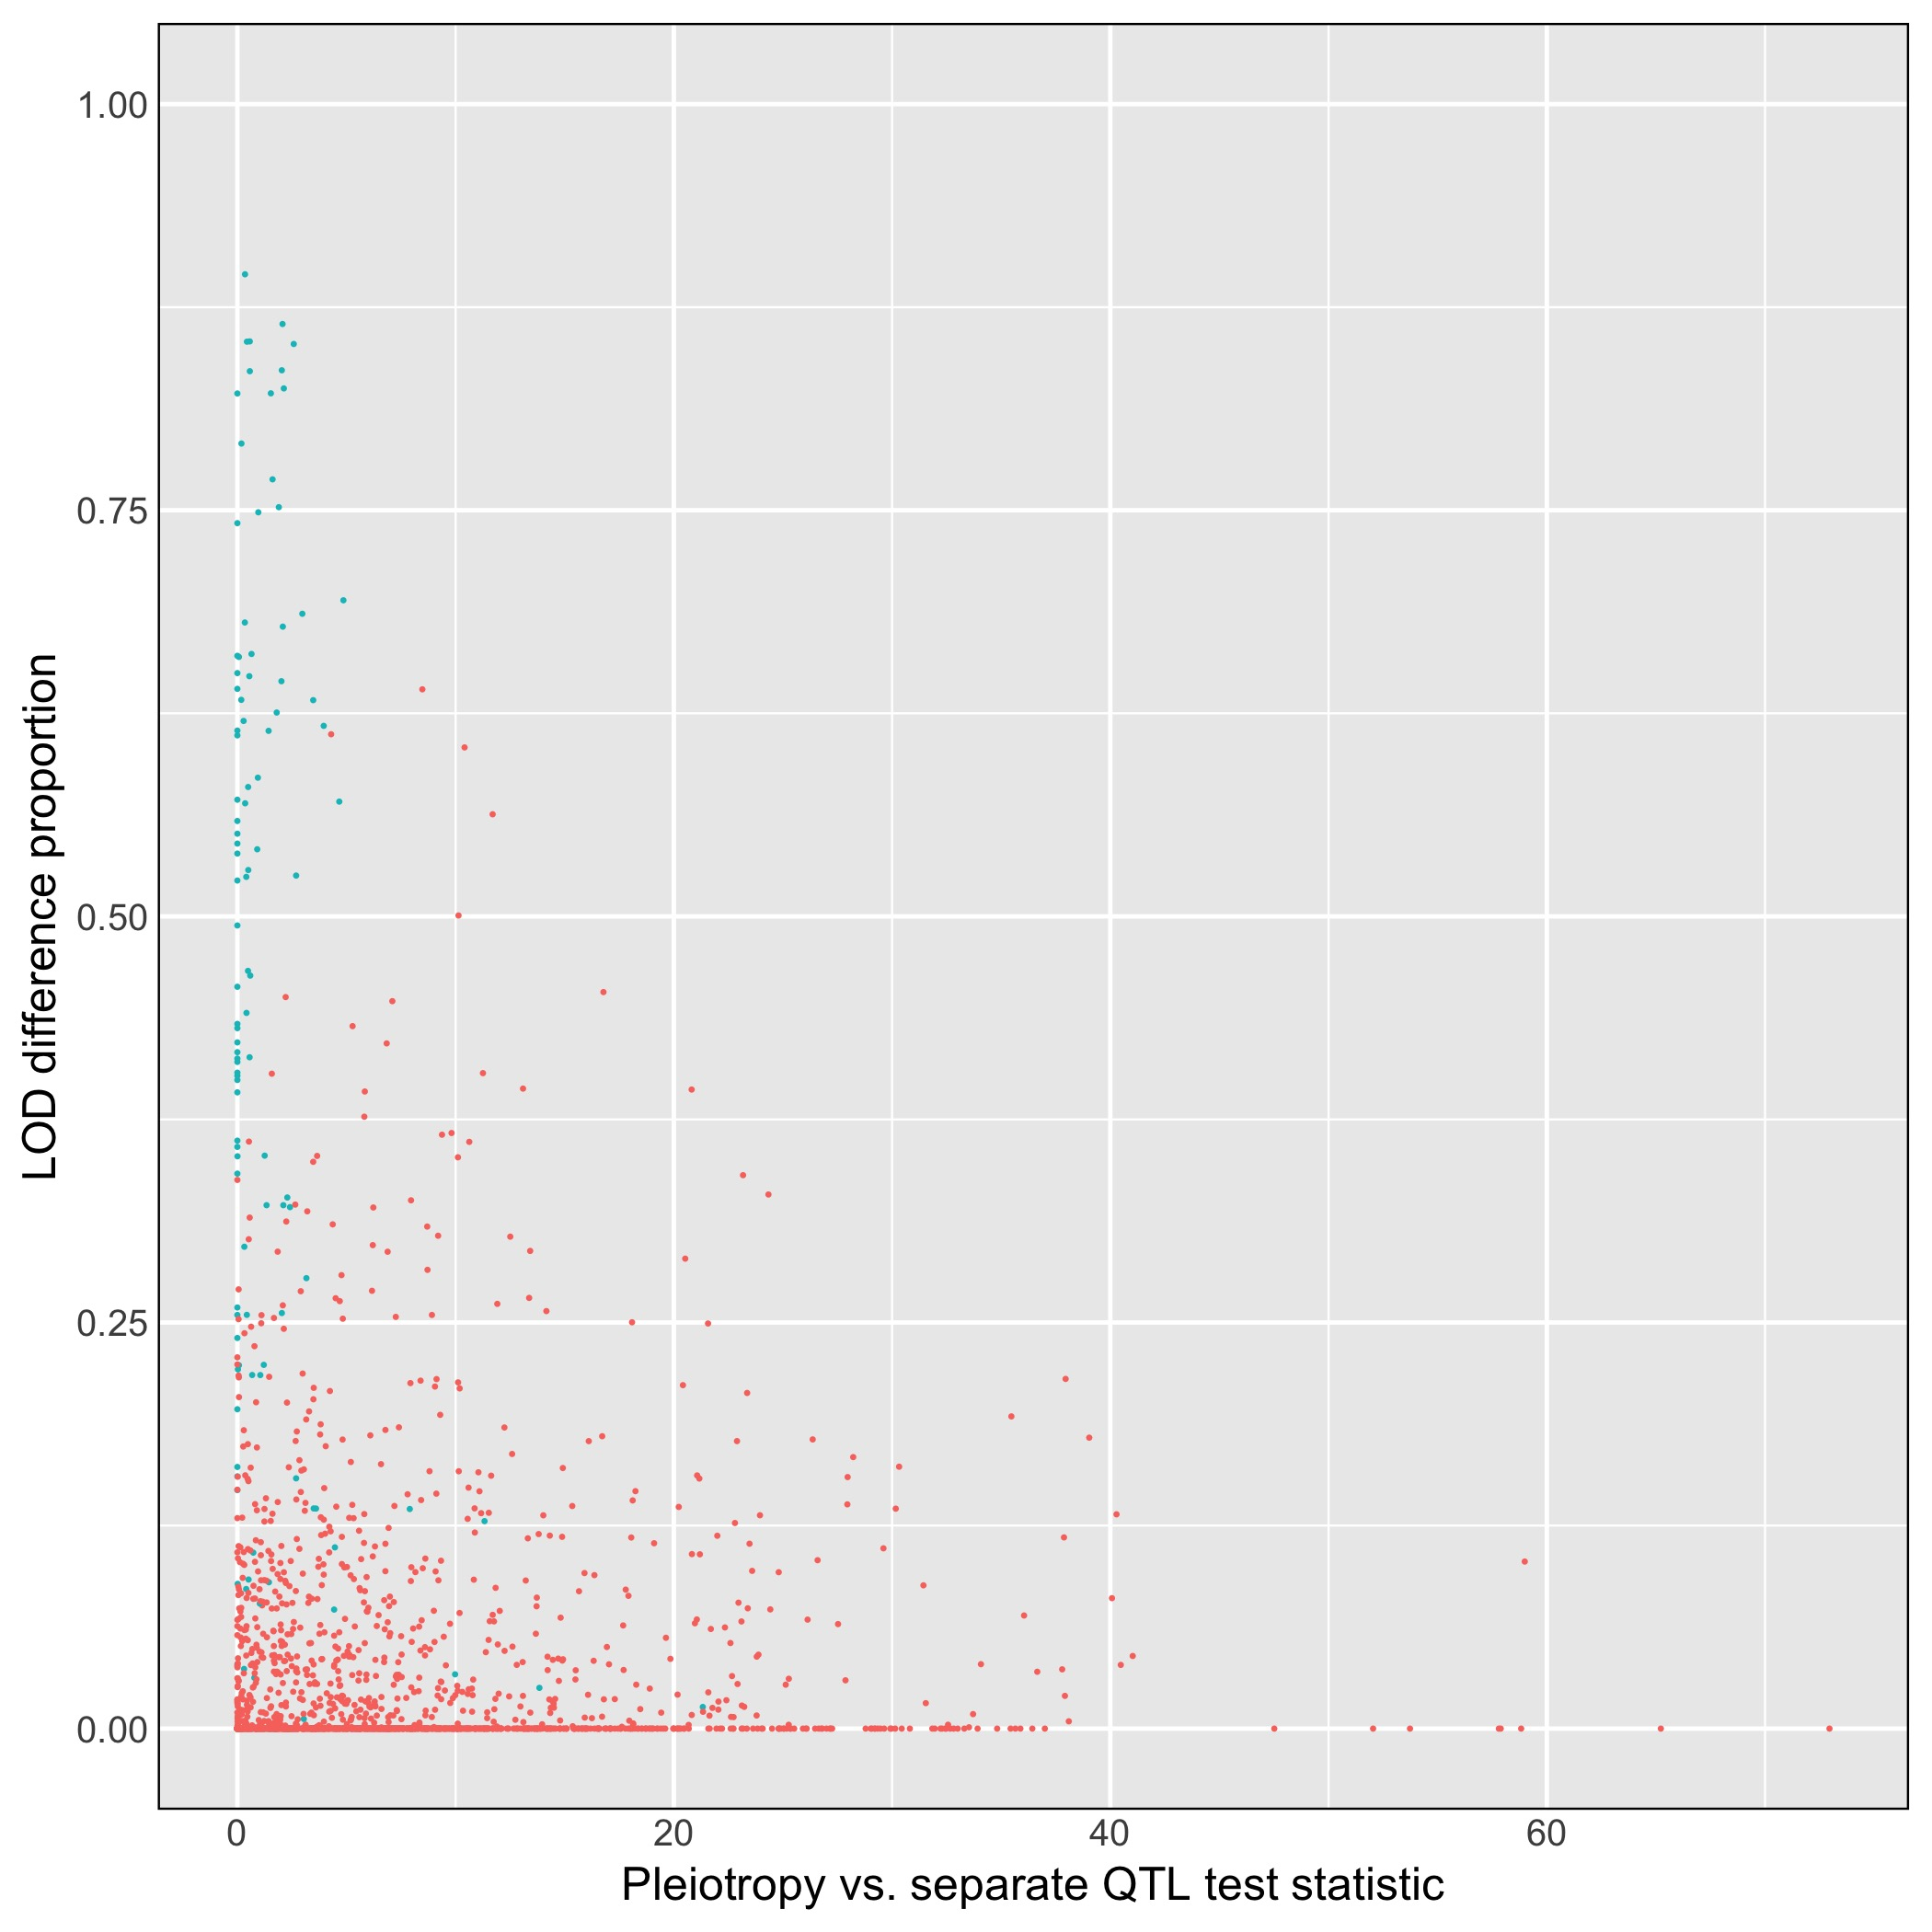
\includegraphics[width = 0.7\textwidth]{lod-diff-prop-v-lrt.jpg}
    \caption{LOD difference proportion against pleiotropy vs. separate QTL test statistics for 1911 pairs of traits. Each point represents a single pair. Pairs that involve local expression trait Hnf4a are colored blue, while all others are colored red. Note the high prevalence of blue points in the upper left quadrant of the figure. These points, with low values of the pleiotropy vs. separate QTL test statistic and high values of LOD difference proportion, are consistent with Hnf4a transcript levels mediating the effect of Hnf4a genetic variants affecting nonlocal transcript abundances.}
    \label{fig:lod-diff-prop-v-lrt-all}
\end{figure}

\subsection{Local gene analyses}

To more thoroughly examine the relationships across the 13 local genes, we created 13 plots of LOD difference proportion (from the mediation analyses) against pleiotropy vs. separate QTL test statistic. They reveal common patterns. First, we see no points in the upper right quadrant of each plot. This tells us that those nonlocal genes with high values of pleiotropy vs. separate QTL test statistic have low values of LOD difference proportion. Similarly, those nonlocal genes with high values of LOD difference proportion tend to have small values of the pleiotropy vs. separate QTL test statistic. Finally, some trait pairs demonstrate low values of both the LOD difference proportion and pleiotropy vs. separate QTL test statistic. This observation suggests that, for a given local expression trait, these pairs are not mediated by the local expression trait yet they arise from a shared locus. 

In comparing the \emph{Hnf4a} plot (Figure \ref{fig:hnf4a}) with the other 12 plots (Figure \ref{fig:nothnf4a-12}), we see that none of the 12 plots in Figure \ref{fig:nothnf4a-12} closely resembles Figure \ref{fig:hnf4a}. Serinc3, Stk4, Neurl2, and Cdh22 are closest in appearance to the plot of Hnf4a. However, each of Serinc3, Stk4, Neurl2, and Cdh22 has very few points with LOD difference proportion above 0.5, while Hnf4a has many points with LOD difference proportion above 0.5.





\begin{figure}
    \centering
    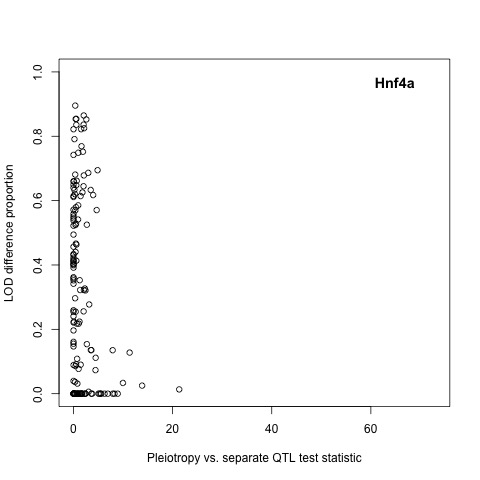
\includegraphics[width = \textwidth]{baseR-Hnf4a.jpg}
    \caption{Scatter plot of LOD difference proportion against pleiotropy vs. separate QTL test statistic value for 147 pairs of expression traits. Each pair pairs Hnf4a as the local gene expression trait with one of the 147 nonlocal traits. 18 of 147 nonlocal traits have pleiotropy vs. separate QTL test statistic values greater than 5, which suggests that approximately 128 of 147 nonlocal traits share a pleiotropic QTL with Hnf4a. Note also the considerable proportion of points with LOD difference proportion greater than 0.5.}
    \label{fig:hnf4a}
\end{figure}

\begin{figure}
    \centering
    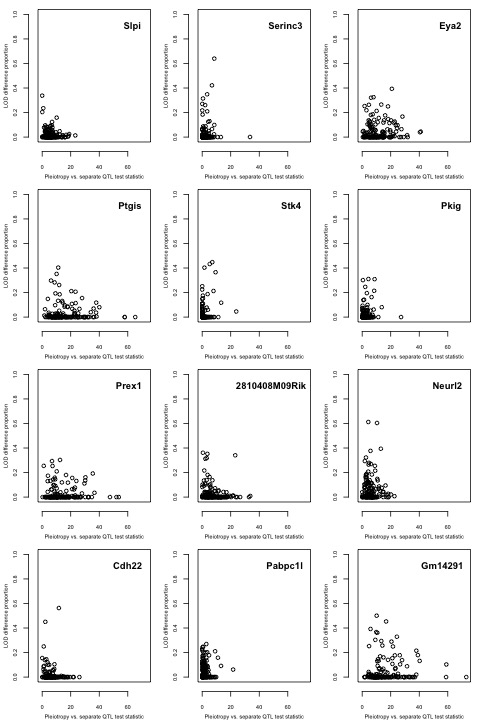
\includegraphics[height = 0.9\textheight]{baseR-12.jpg}
    \caption{Scatter plots of LOD difference proportion against pleiotropy vs. separate QTL test statistic for each of 12 local gene expression traits. Each plot is labeled with the local gene expression trait. Each plot contains 147 points, resulting from analyses involving the labeled local gene expression trait and each of the 147 nonlocal gene expression traits.}
    \label{fig:nothnf4a-12}
\end{figure}

% latex table generated in R 3.5.1 by xtable 1.8-3 package
% Wed Dec 19 10:50:32 2018
\begin{table}[ht]
\centering
\begin{tabular}{lc}
  \hline
 Local gene & Number of nonlocal gene expression traits \\ 
  \hline
2810408M09Rik &   3 \\ 
  Cdh22 &   4 \\ 
  Eya2 &   4 \\ 
  Gm14291 &   5 \\ 
  Hnf4a &  89 \\ 
  Neurl2 &  15 \\ 
  Pabpc1l &   4 \\ 
  Pkig &   2 \\ 
  Prex1 &   5 \\ 
  Ptgis &   3 \\ 
  Serinc3 &   7 \\ 
  Slpi &   1 \\ 
  Stk4 &   5 \\ 
   \hline
\end{tabular}
\caption{Number of nonlocal gene expression traits for which each local gene expression trait is the strongest mediator.}
\label{tab:med-count}
\end{table}

\subsection{Nonlocal gene analyses}

Scatter plots of LOD difference proportion values against pleiotropy vs. separate QTL test statistics for each of the 147 nonlocal expression traits demonstrated multiple patterns. Eighty-nine nonlocal genes' plots showed Hnf4a to have the greatest value, among the 13 putative mediators, of the LOD difference proportion statistic. In many cases, Hnf4a's LOD difference proportion statistic was at least twice that of any of the other 12 local gene expression levels.

\begin{figure}
    \centering
    \caption{Scatter plots for four nonlocal expression traits. Each plot features 13 points, one for each local gene expression trait. The y axis denotes LOD difference proportion values, while the x axis corresponds to pleiotropy vs. separate QTL test statistics. Blue points represent the pairing with local gene expression trait Hnf4a. Red points represent the other 12 local gene expression traits.}
    \begin{subfigure}[t]{.45\textwidth}
        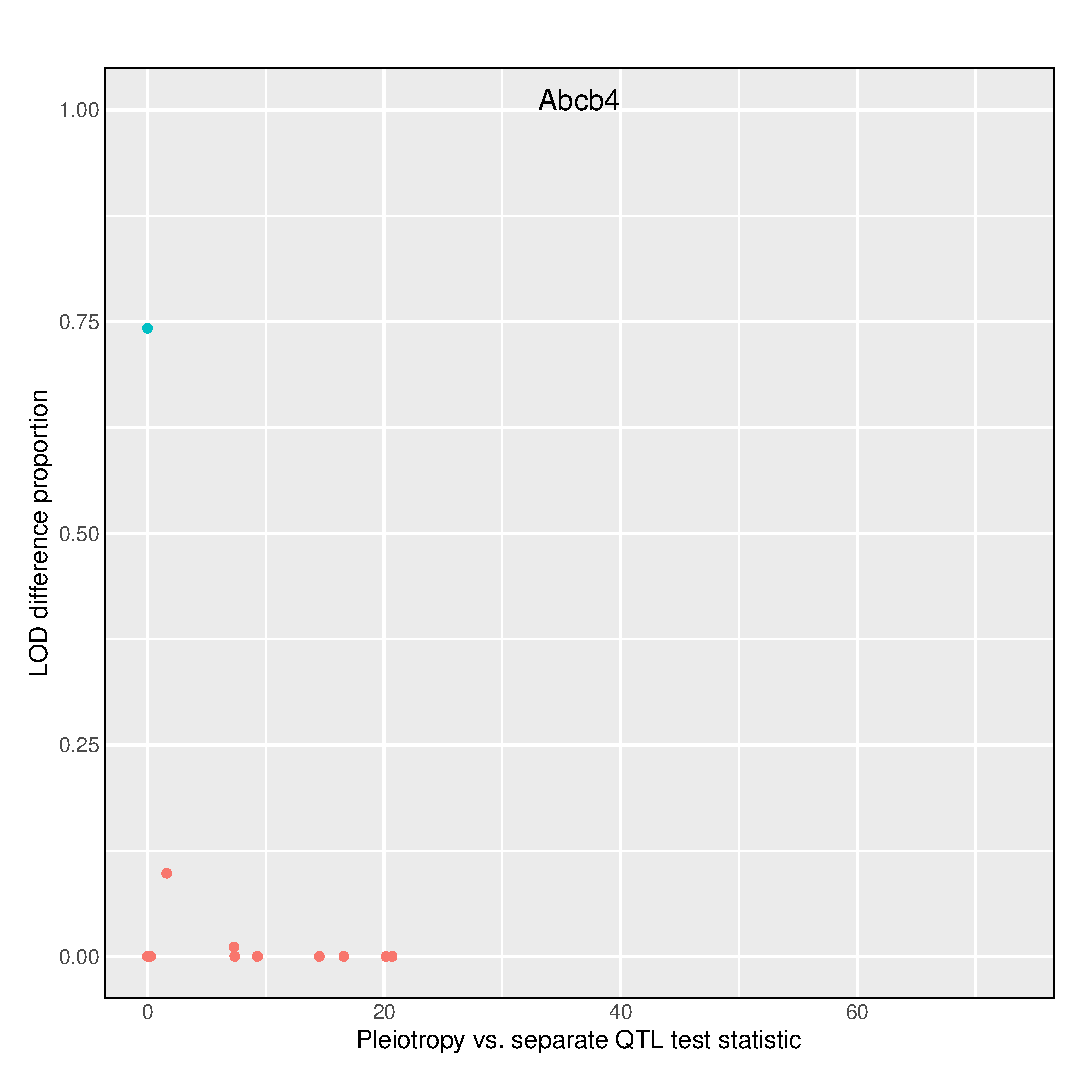
\includegraphics[width = \textwidth]{nonlocal-scatter_97.eps}
        \caption{Hnf4a transcript levels mediate Abcb4 transcript levels. The high LOD difference proportion and the very small pleiotropy vs. separate QTL test statistic together provide evidence that Hnf4a mediates Abcb4 transcript levels.}
    \end{subfigure}
    \begin{subfigure}[t]{.45\textwidth}
        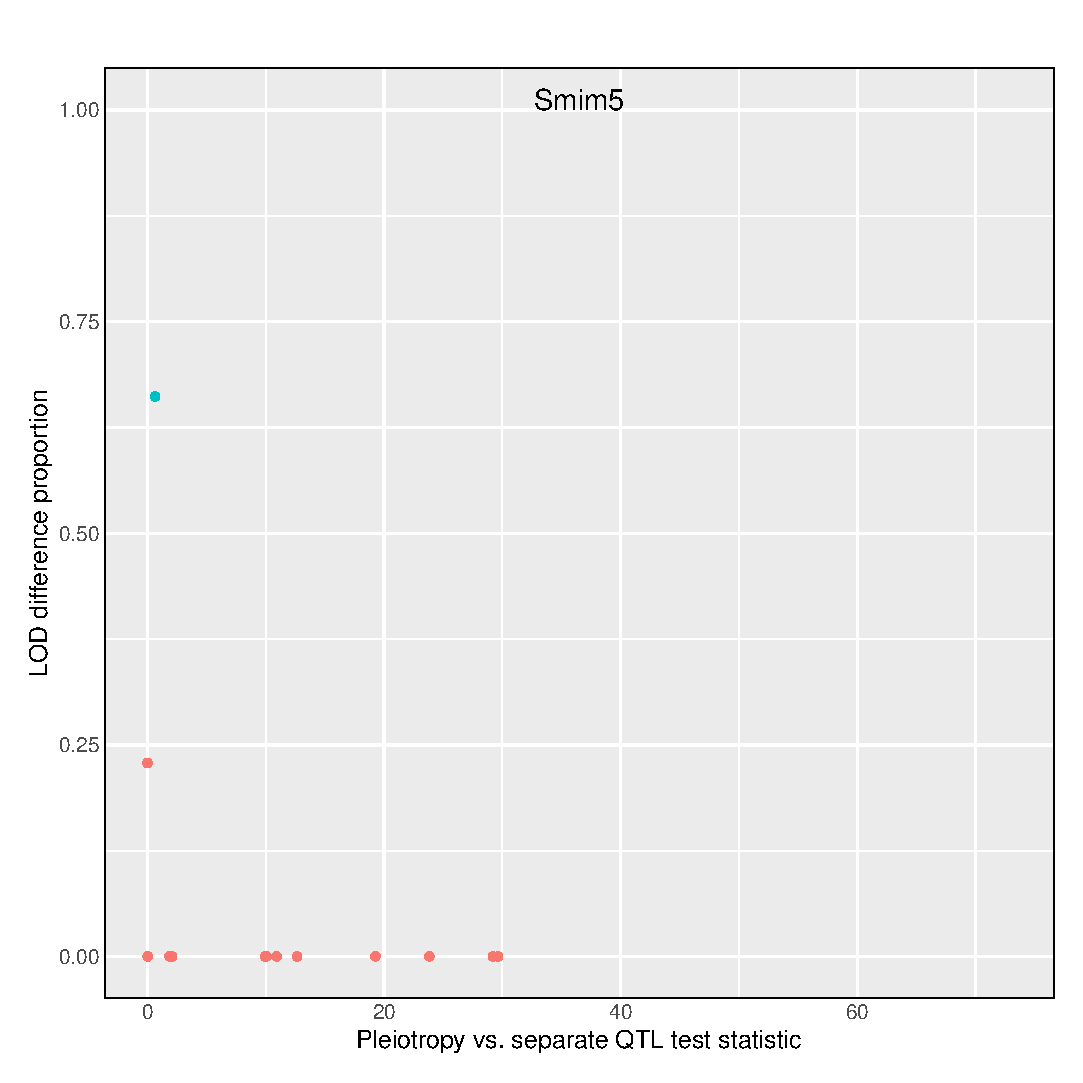
\includegraphics[width = \textwidth]{nonlocal-scatter_105.eps}
        \caption{Hnf4a transcript levels mediate Smim5 transcript levels. The high LOD difference proportion and the very small pleiotropy vs. separate QTL test statistic together provide evidence that Hnf4a mediates Smim5 transcript levels.}
    \end{subfigure}
    \begin{subfigure}[t]{.45\textwidth}
        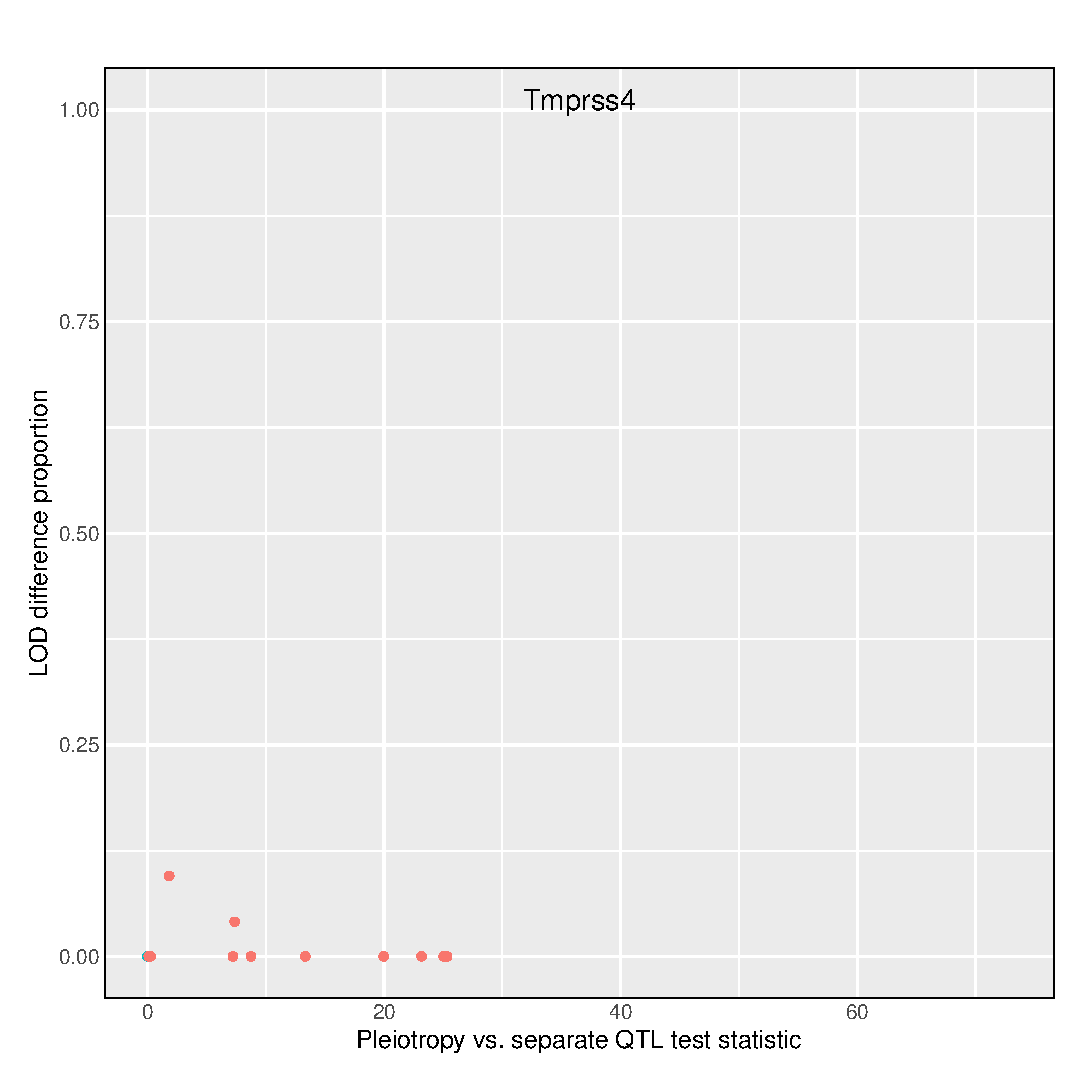
\includegraphics[width = \textwidth]{nonlocal-scatter_64.eps}
        \caption{Tmprww4 transcript levels are not mediated by any of the 13 local gene expression traits. However, several local gene expression traits arise from separate QTL, as evidenced by their large (greater than 5) values of the pleiotropy vs. separate QTL test statistic.}
    \end{subfigure}
    \begin{subfigure}[t]{.45\textwidth}
        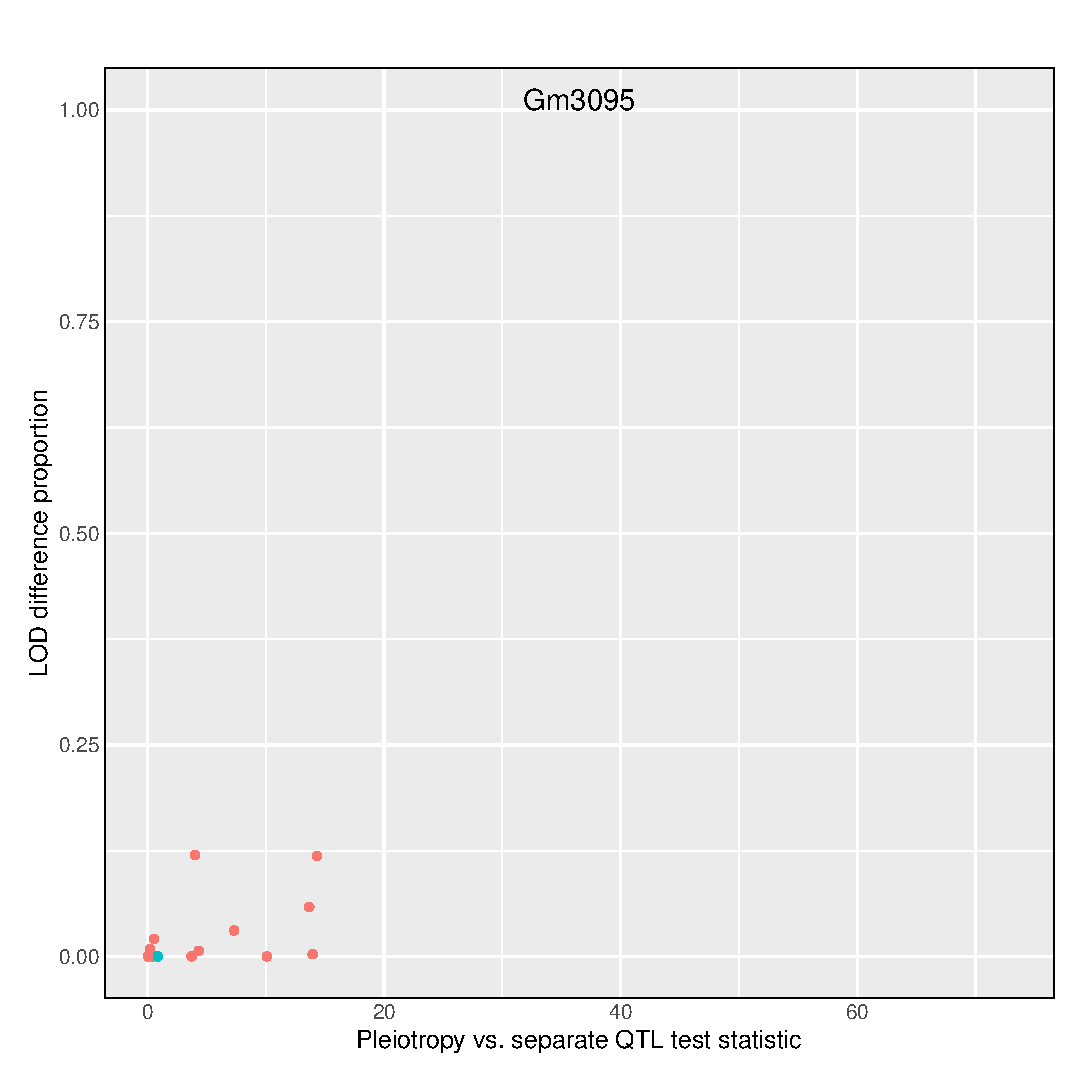
\includegraphics[width = \textwidth]{nonlocal-scatter_141.eps}
        \caption{Gm3095 transcript levels are not mediated by any of the 13 local genes. The tests of pleiotropy vs. separate QTL demonstrate evidence of separate QTL for some local expression traits when paired with Gm3095.}
    \end{subfigure}
    \label{fig:my_label}
\end{figure}





\section{Discussion}

Our pairwise analyses with both mediation analyses and tests of pleiotropy vs. separate QTL provide additional evidence for the importance of Hnf4a in the biology of the Chromosome 2 hotspot in pancreatic islet cells. Our analyses, and, specifically, the test of pleiotropy vs. separate QTL, may be more useful when studying nonlocal traits that map to a hotspot yet don't show strong evidence of mediation by local expression traits. In such a setting, the test of pleiotropy vs. separate QTL can, at least, provide some information about the genetic architecture at the hotspot. 

On the other hand, mediation analyses, when they provide evidence for mediation of a nonlocal trait by a local expression trait, are more informative than the test of pleiotropy vs. separate QTL. 








We found that, when there is a well-defined mediator, between a DNA variant and a nonlocal expression trait, regression-based mediation analyses identify the relationship. However, in those cases in which no clear mediator exists, our test of pleiotropy vs. separate QTL provides valuable information in the dissection of QTL hotspots. 







\printbibliography

\begin{figure}
\centering
\begin{subfigure}[t]{.38\textwidth}
\centering
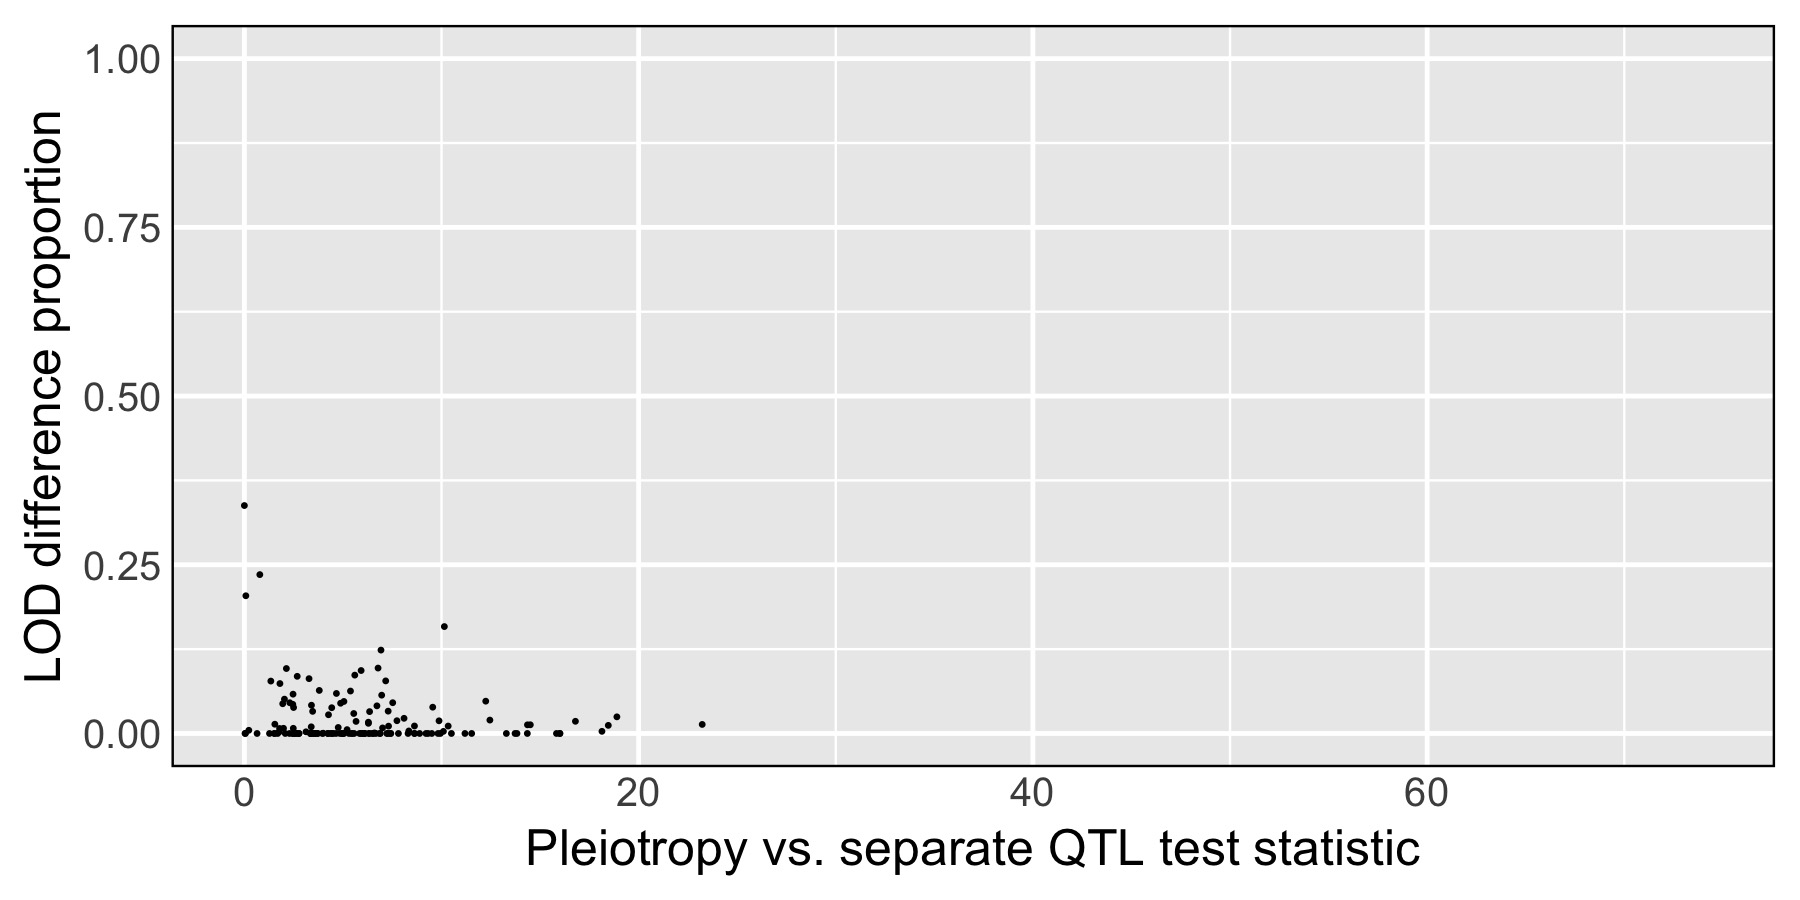
\includegraphics[width=\linewidth]{bar_1.jpg}
        \caption{}\label{fig:fig_a}
\end{subfigure}
%
\begin{subfigure}[t]{.38\textwidth}
\centering
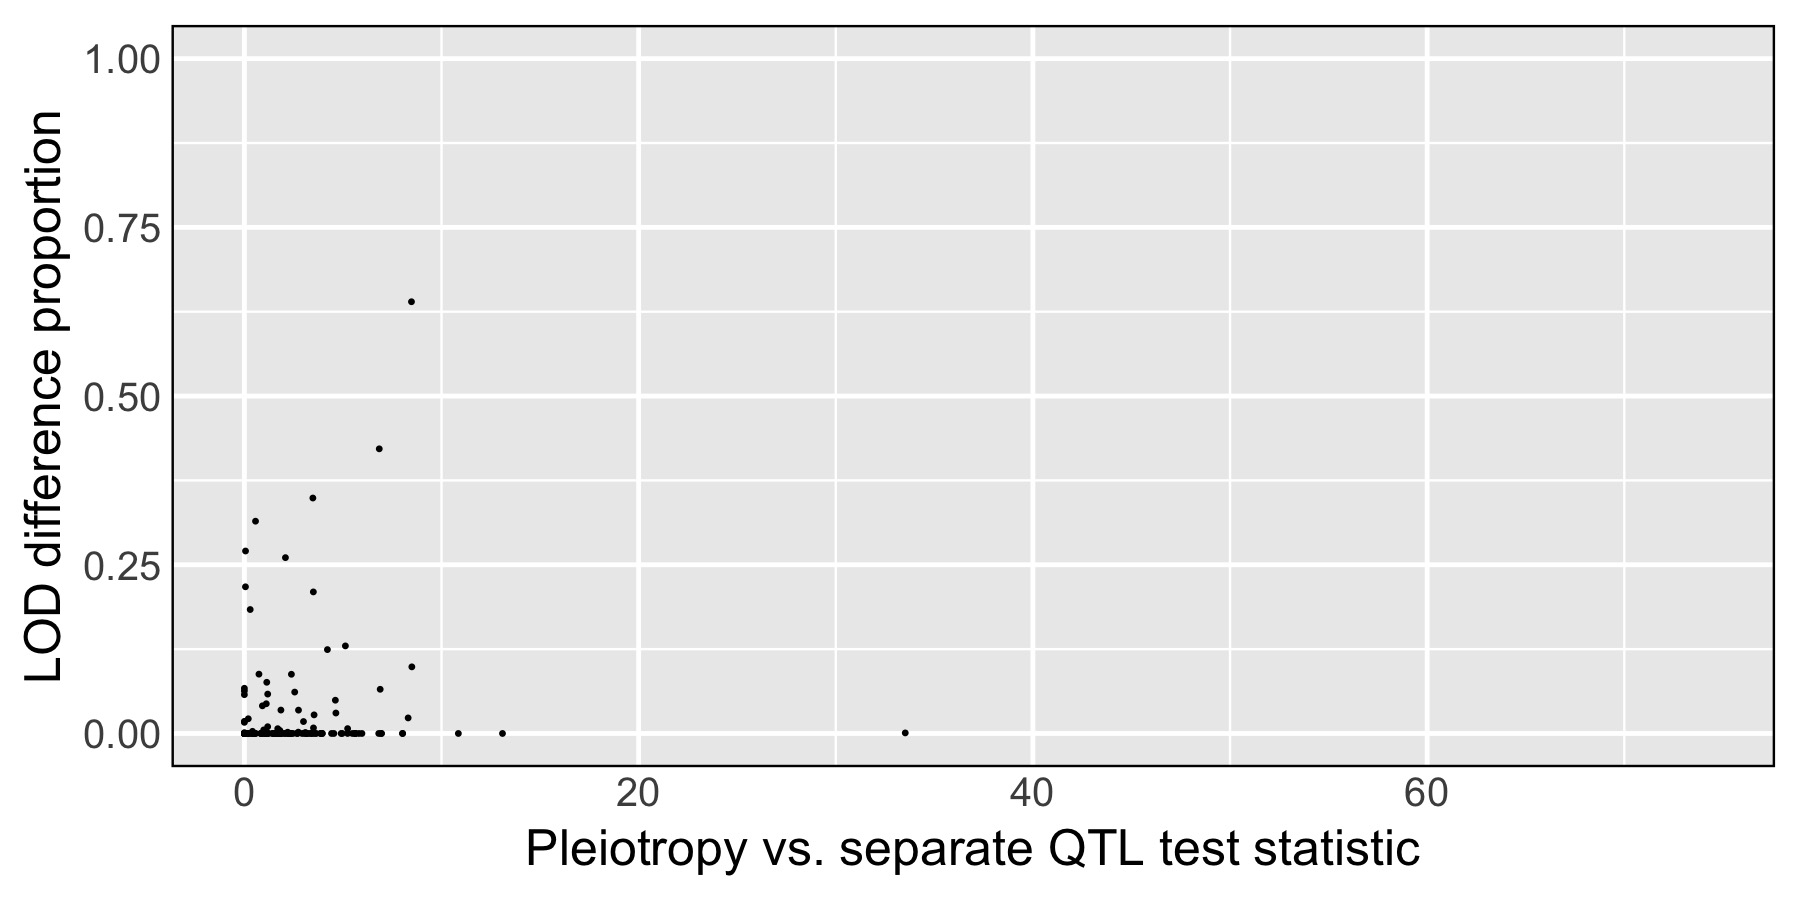
\includegraphics[width=\linewidth]{bar_2.jpg}
\caption{}\label{fig:fig_b}
\end{subfigure}

\medskip

\begin{subfigure}[t]{.38\textwidth}
\centering
\vspace{0pt}% set the real top as the top
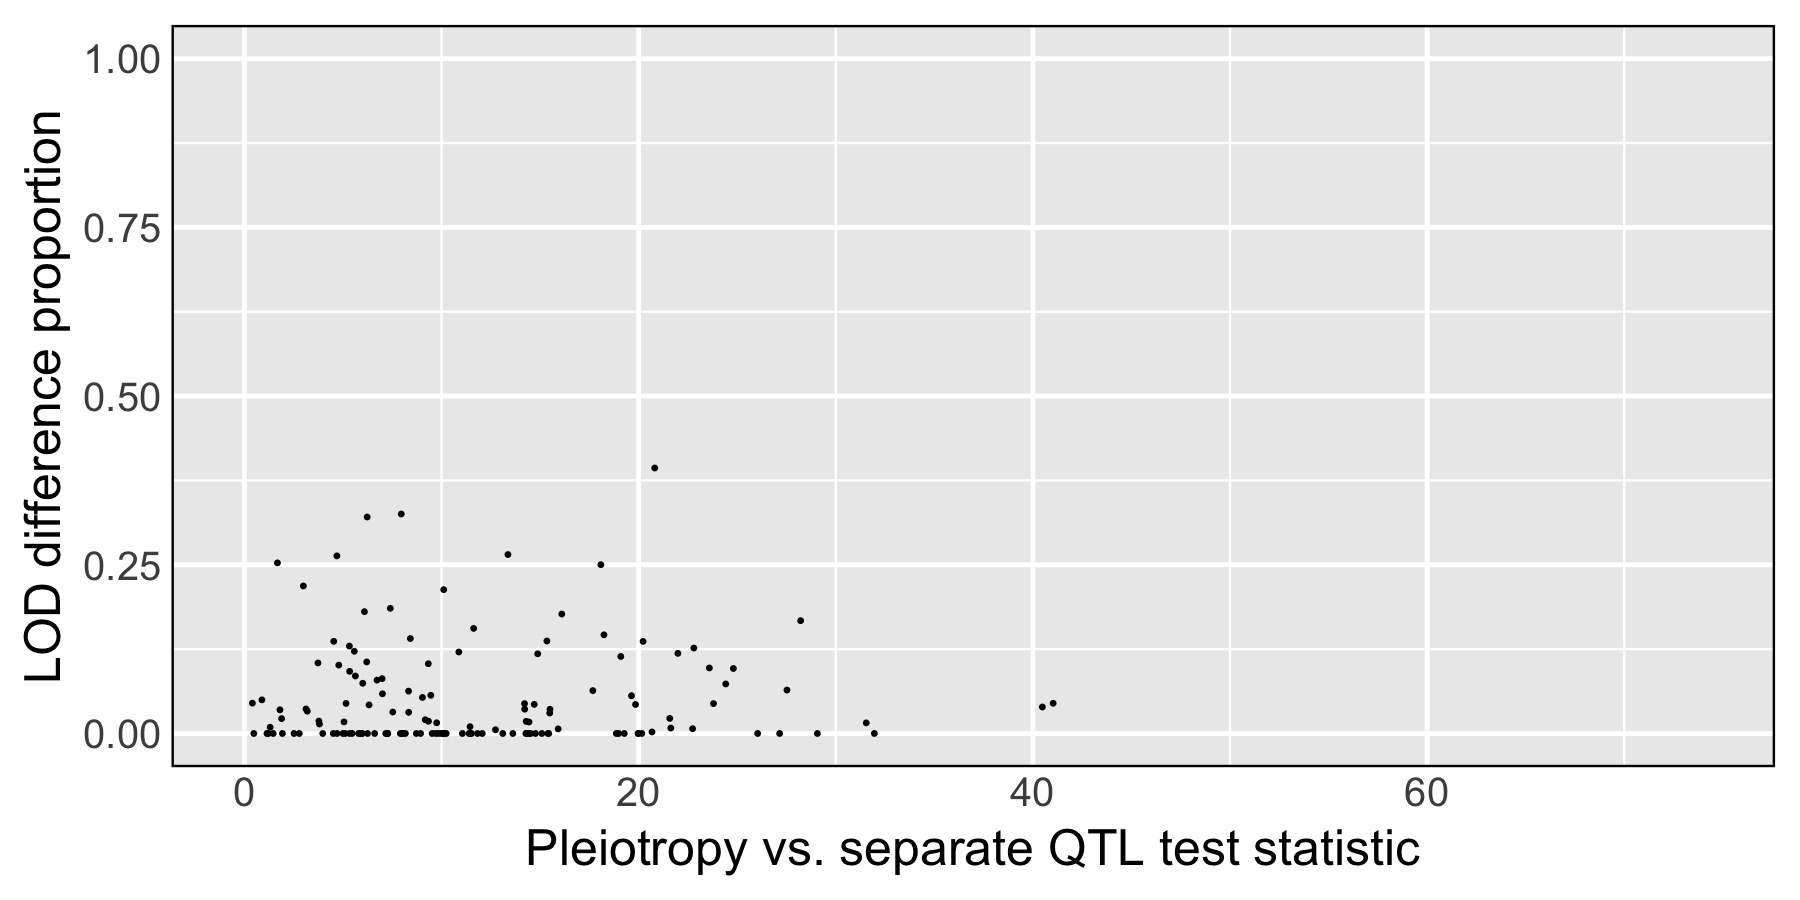
\includegraphics[width=\linewidth]{bar_3.jpg}
\caption{}\label{fig:fig_c}
\end{subfigure}
%
\begin{subfigure}[t]{.38\textwidth}
\centering
\vspace{0pt}% set the real top as the top
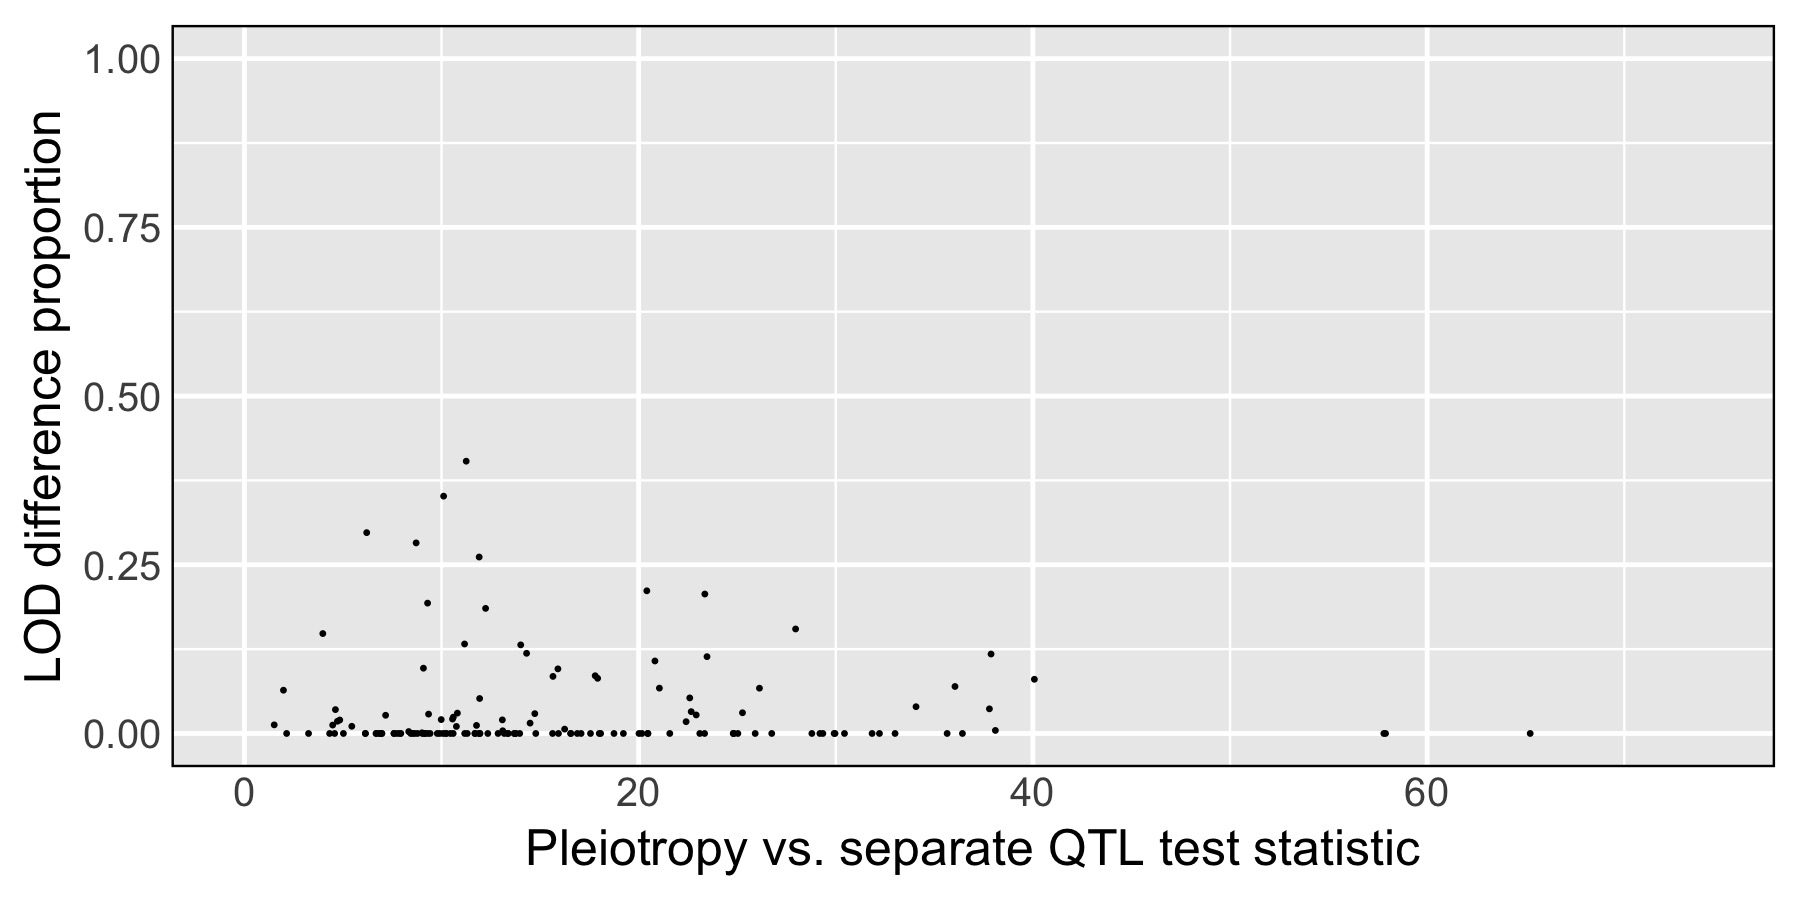
\includegraphics[width=\linewidth]{bar_4.jpg}
\caption{}\label{fig:fig_d}
\end{subfigure}
\begin{subfigure}[t]{.38\textwidth}
\centering
\vspace{0pt}% set the real top as the top
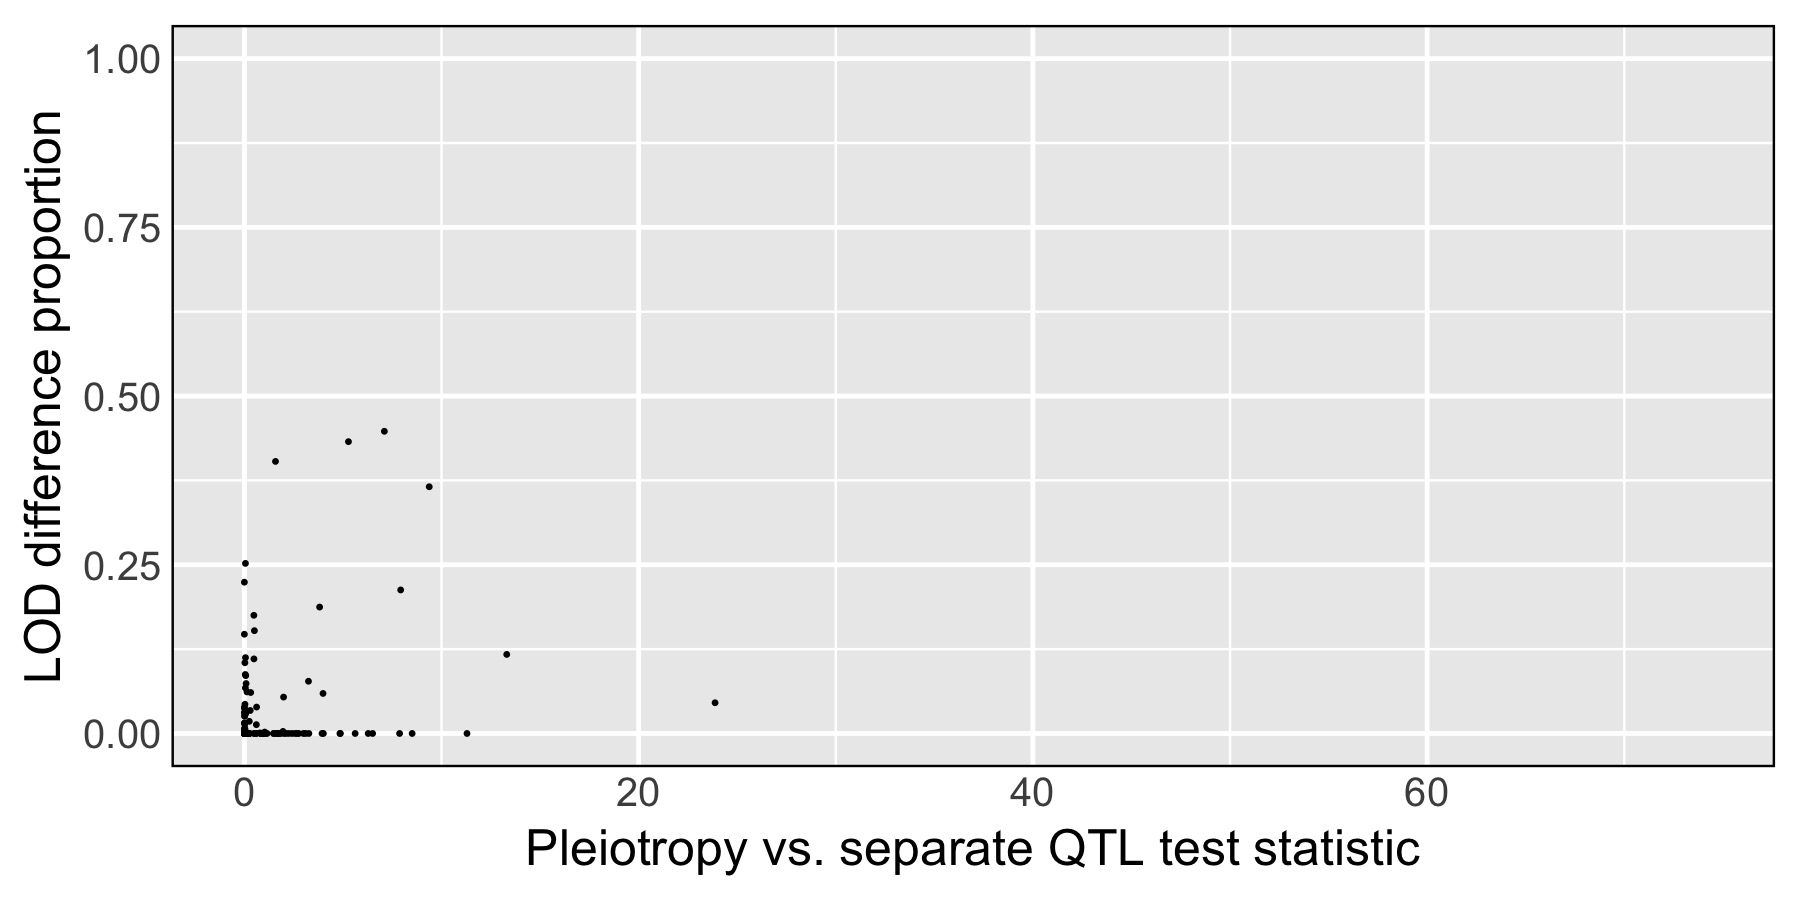
\includegraphics[width=\linewidth]{bar_5.jpg}
\caption{}\label{fig:fig_e}
\end{subfigure}
\begin{subfigure}[t]{.38\textwidth}
\centering
\vspace{0pt}% set the real top as the top
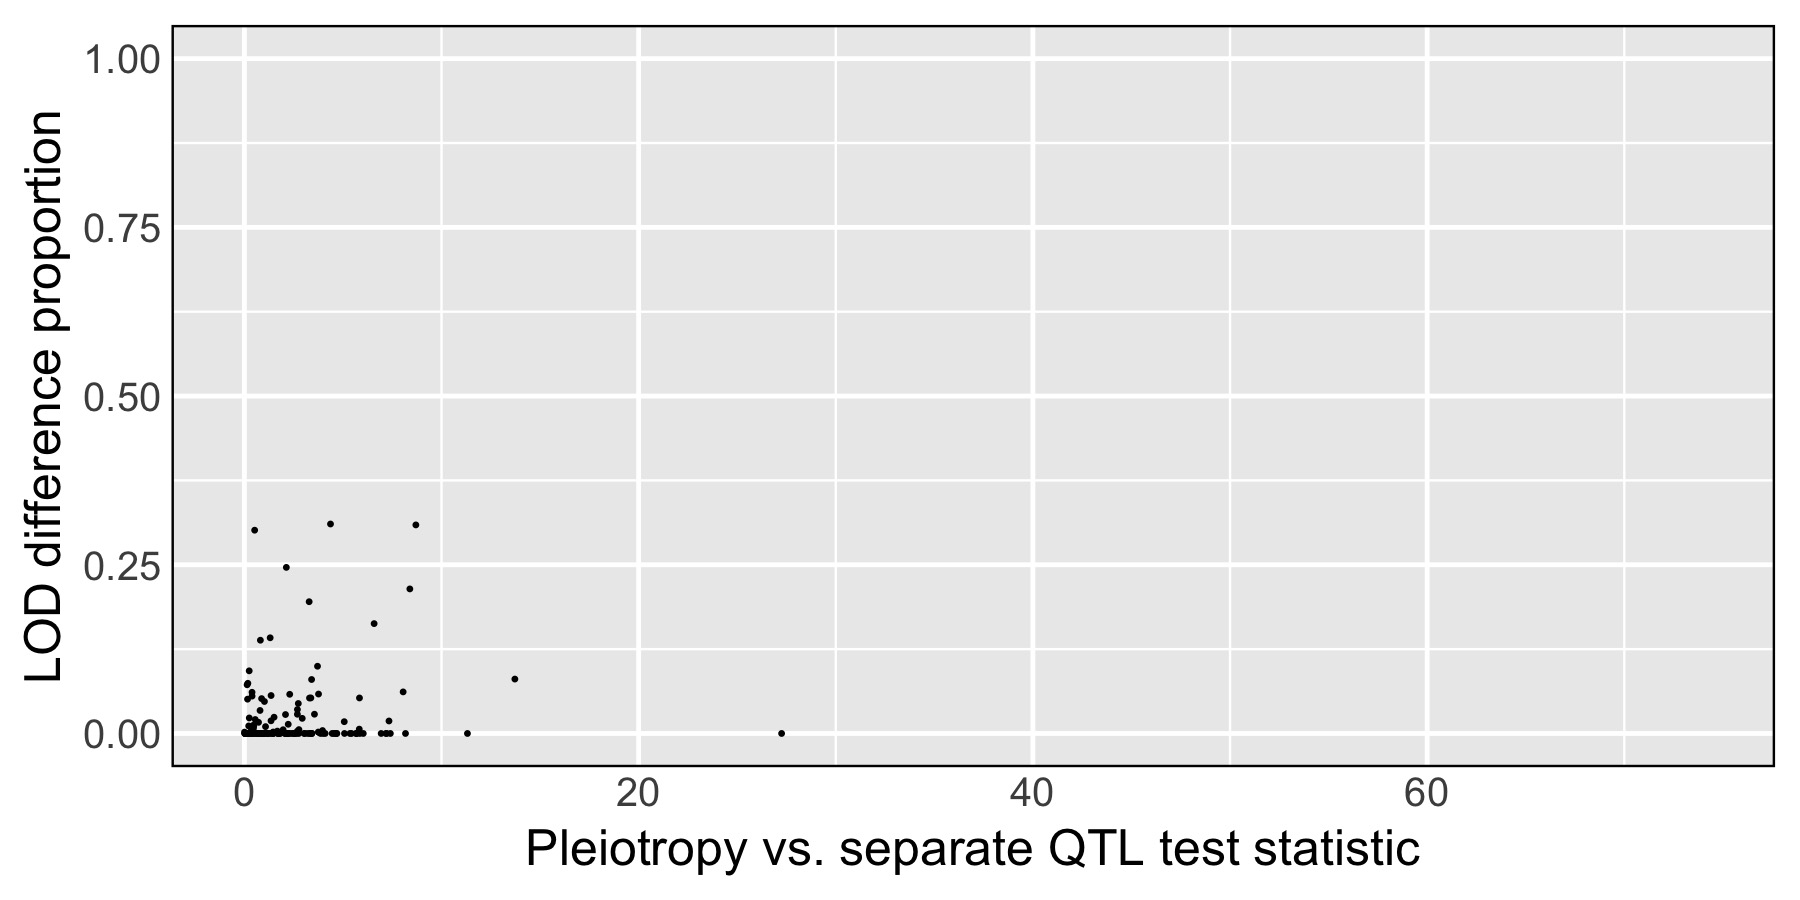
\includegraphics[width=\linewidth]{bar_6.jpg}
\caption{}\label{fig:fig_f}
\end{subfigure}
\begin{subfigure}[t]{.38\textwidth}
\centering
\vspace{0pt}% set the real top as the top
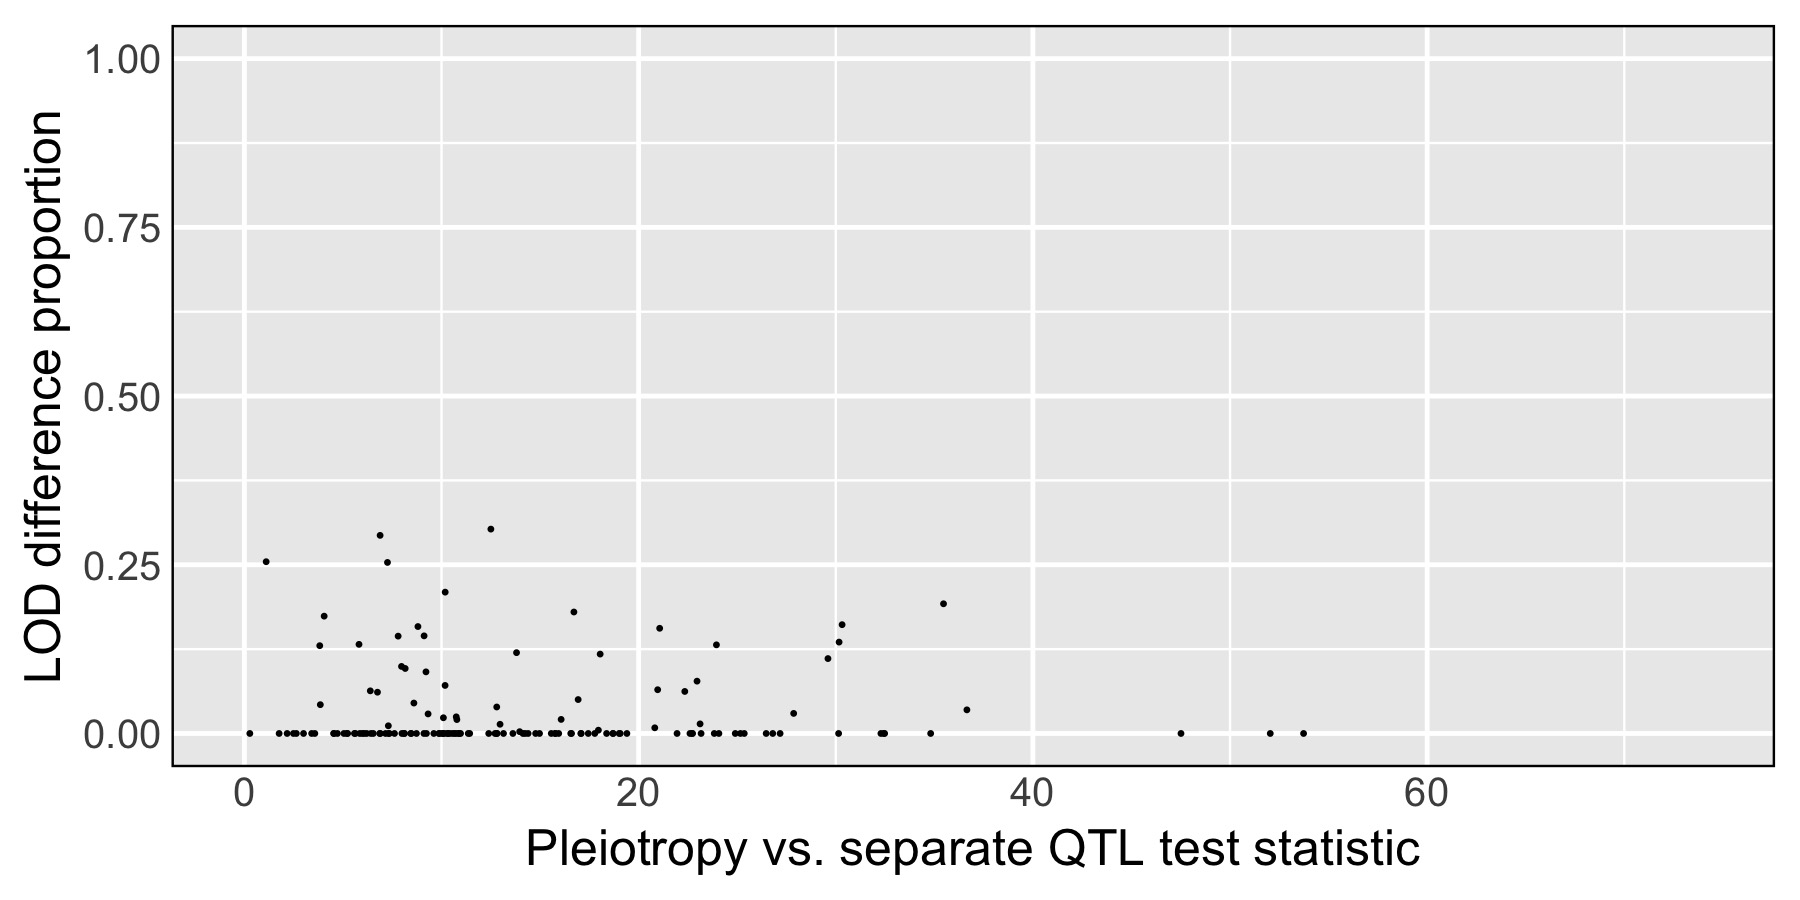
\includegraphics[width=\linewidth]{bar_7.jpg}
\caption{}\label{fig:fig_g}
\end{subfigure}
\begin{subfigure}[t]{.38\textwidth}
\centering
\vspace{0pt}% set the real top as the top
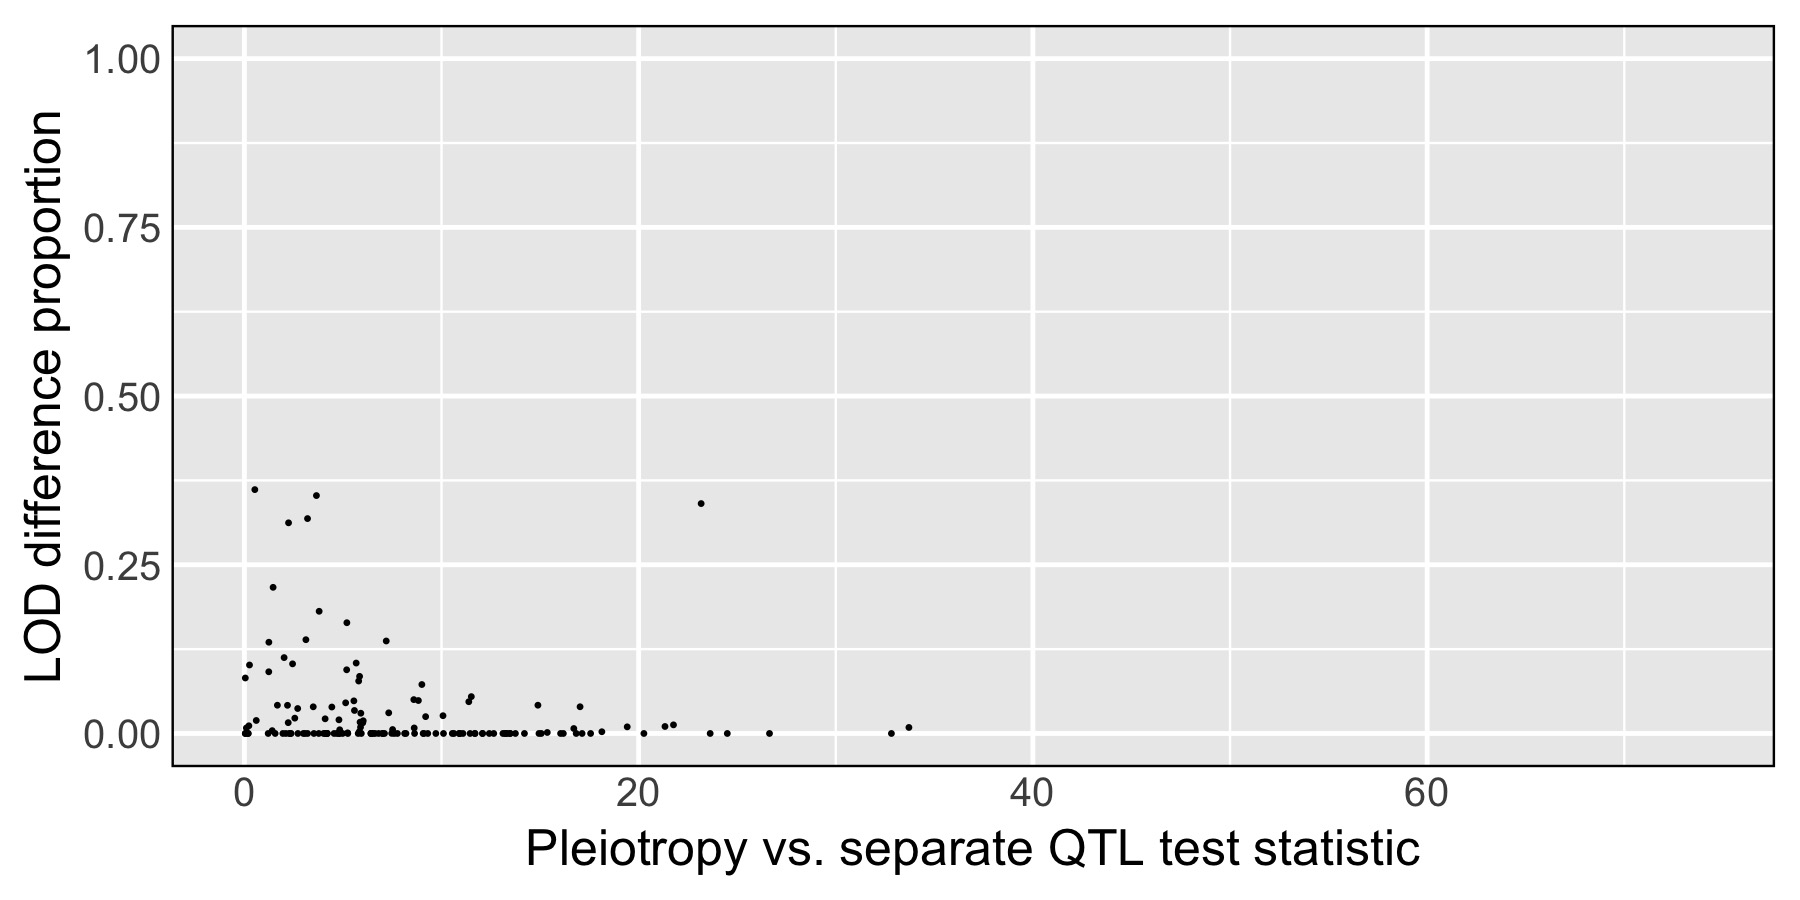
\includegraphics[width=\linewidth]{bar_8.jpg}
\caption{}\label{fig:fig_h}
\end{subfigure}
\begin{subfigure}[t]{.38\textwidth}
\centering
\vspace{0pt}% set the real top as the top
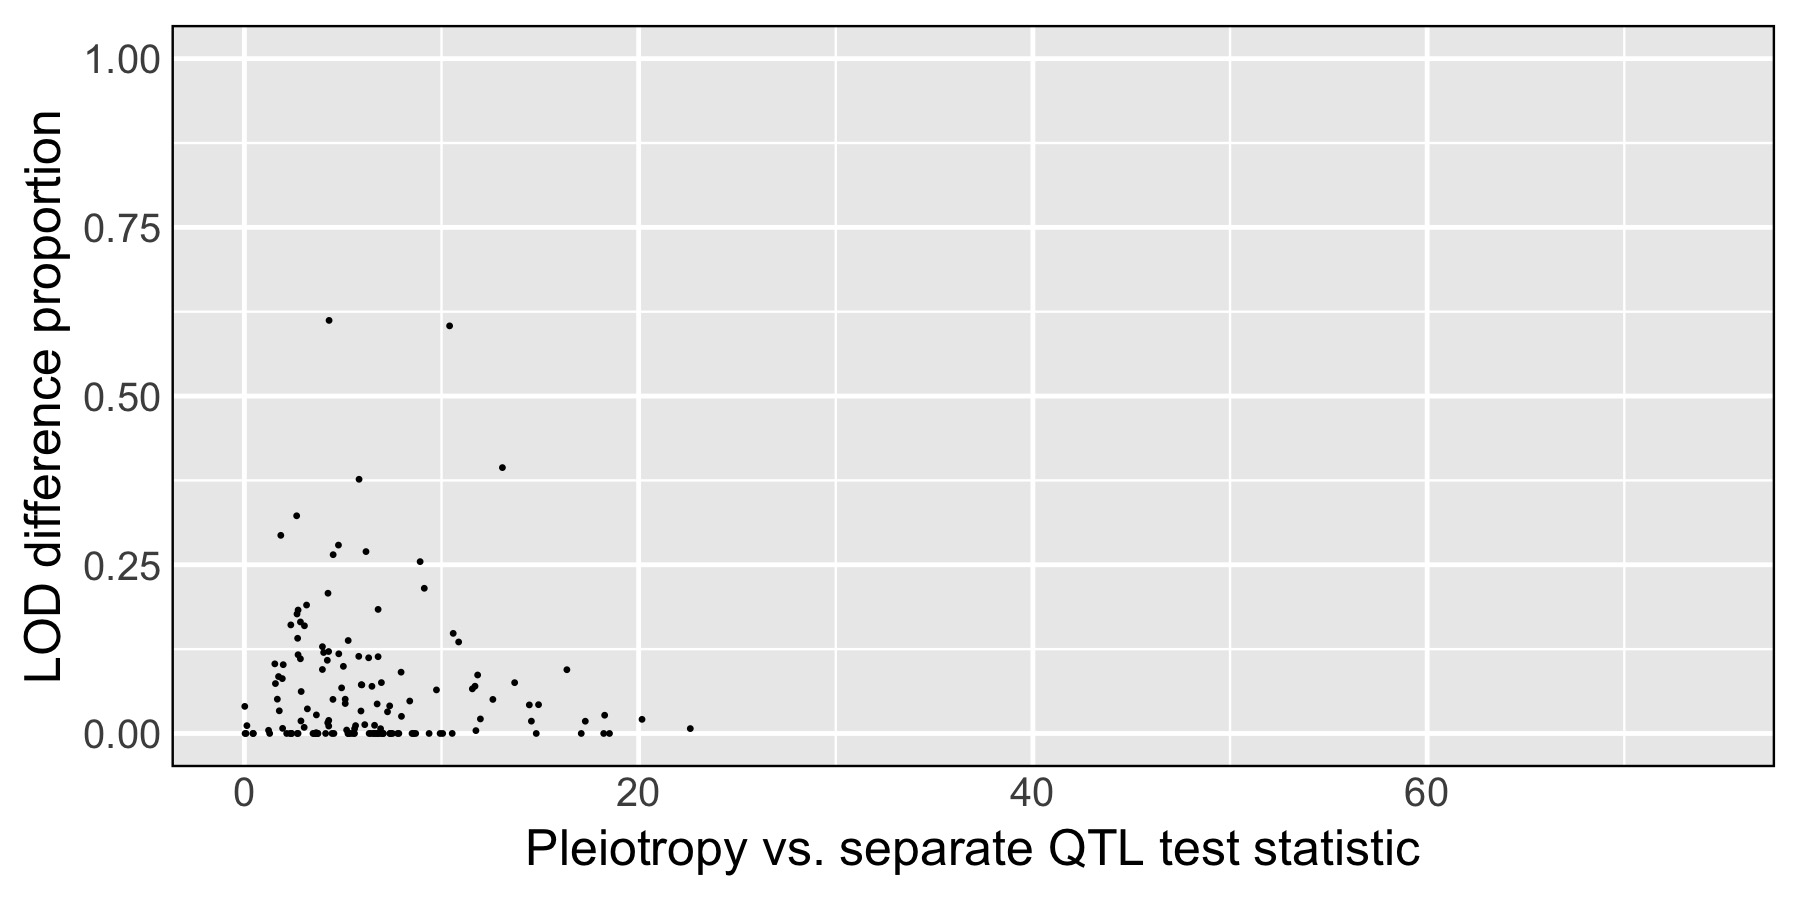
\includegraphics[width=\linewidth]{bar_9.jpg}
\caption{}\label{fig:fig_i}
\end{subfigure}
\begin{subfigure}[t]{.38\textwidth}
\centering
\vspace{0pt}% set the real top as the top
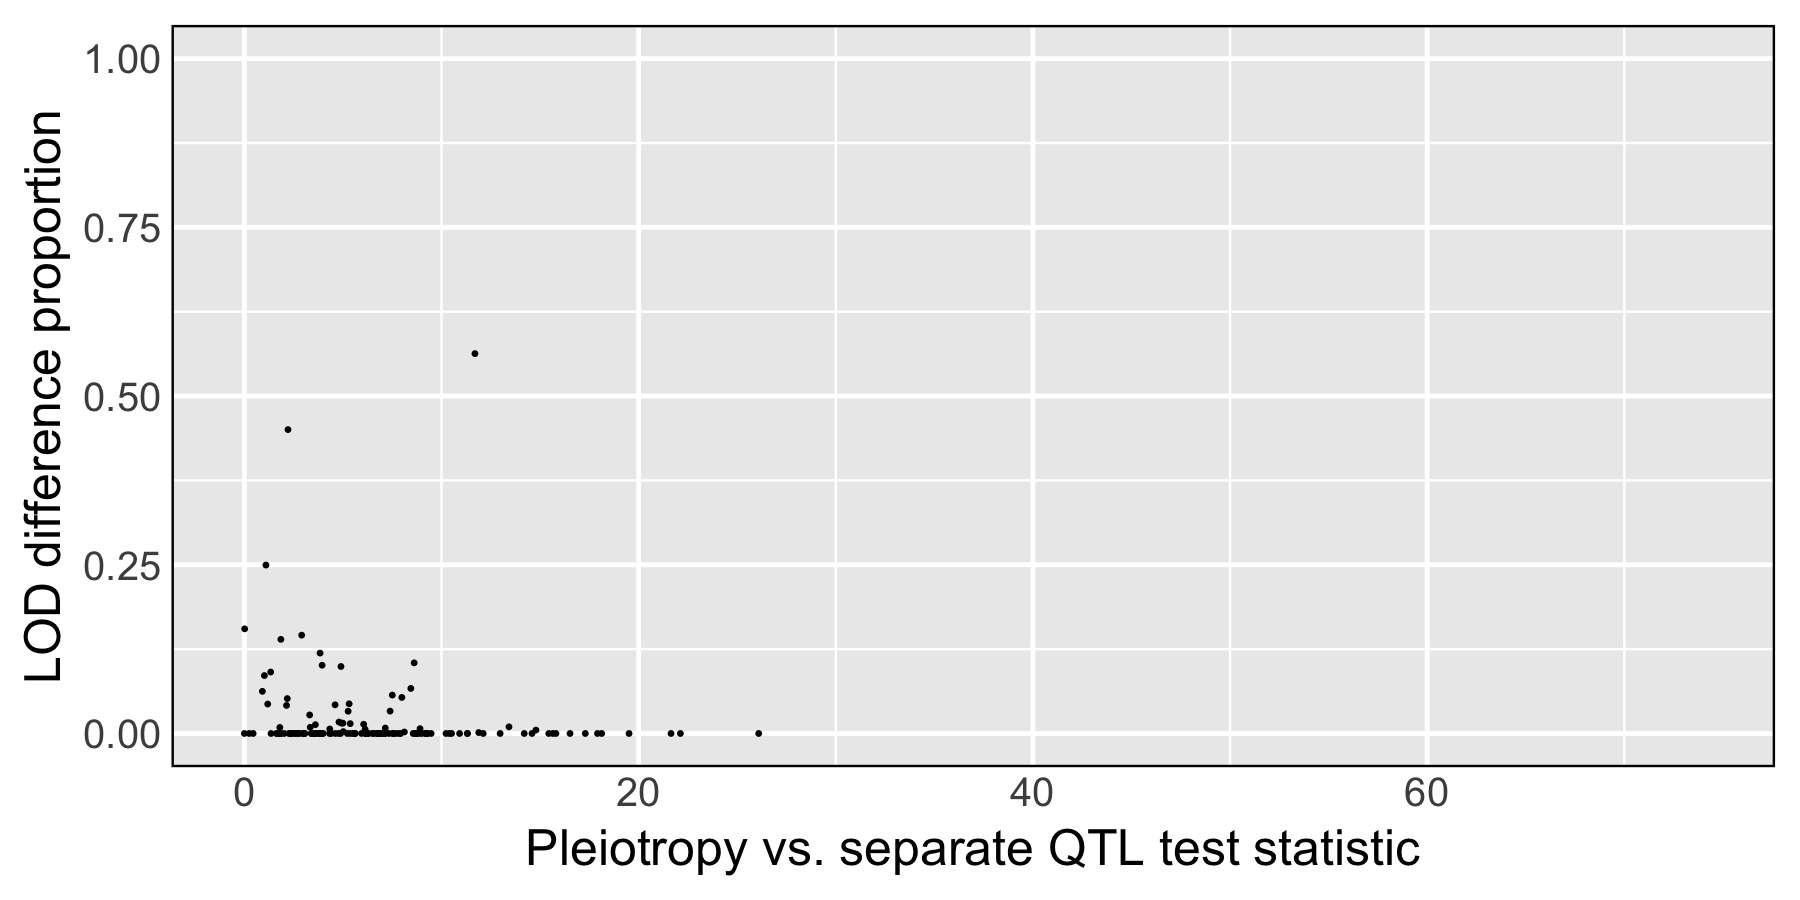
\includegraphics[width=\linewidth]{bar_10.jpg}
\caption{}\label{fig:fig_j}
\end{subfigure}
\begin{subfigure}[t]{.38\textwidth}
\centering
\vspace{0pt}% set the real top as the top
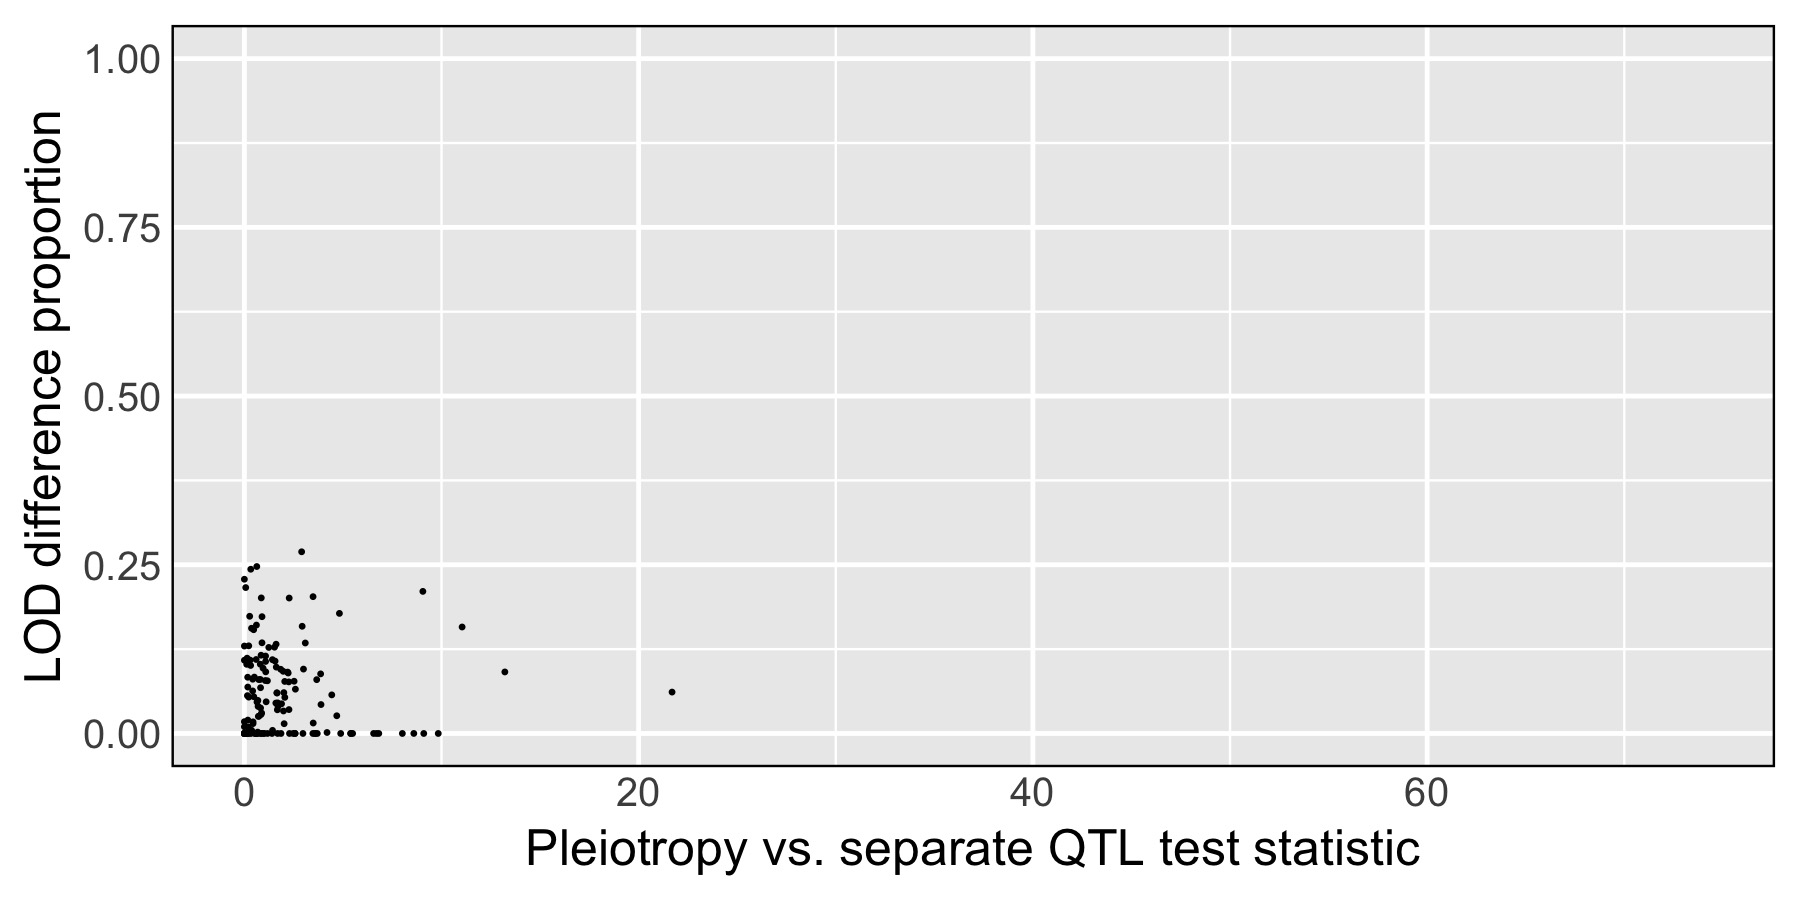
\includegraphics[width=\linewidth]{bar_11.jpg}
\caption{}\label{fig:fig_k}
\end{subfigure}
\begin{subfigure}[t]{.38\textwidth}
\centering
\vspace{0pt}% set the real top as the top
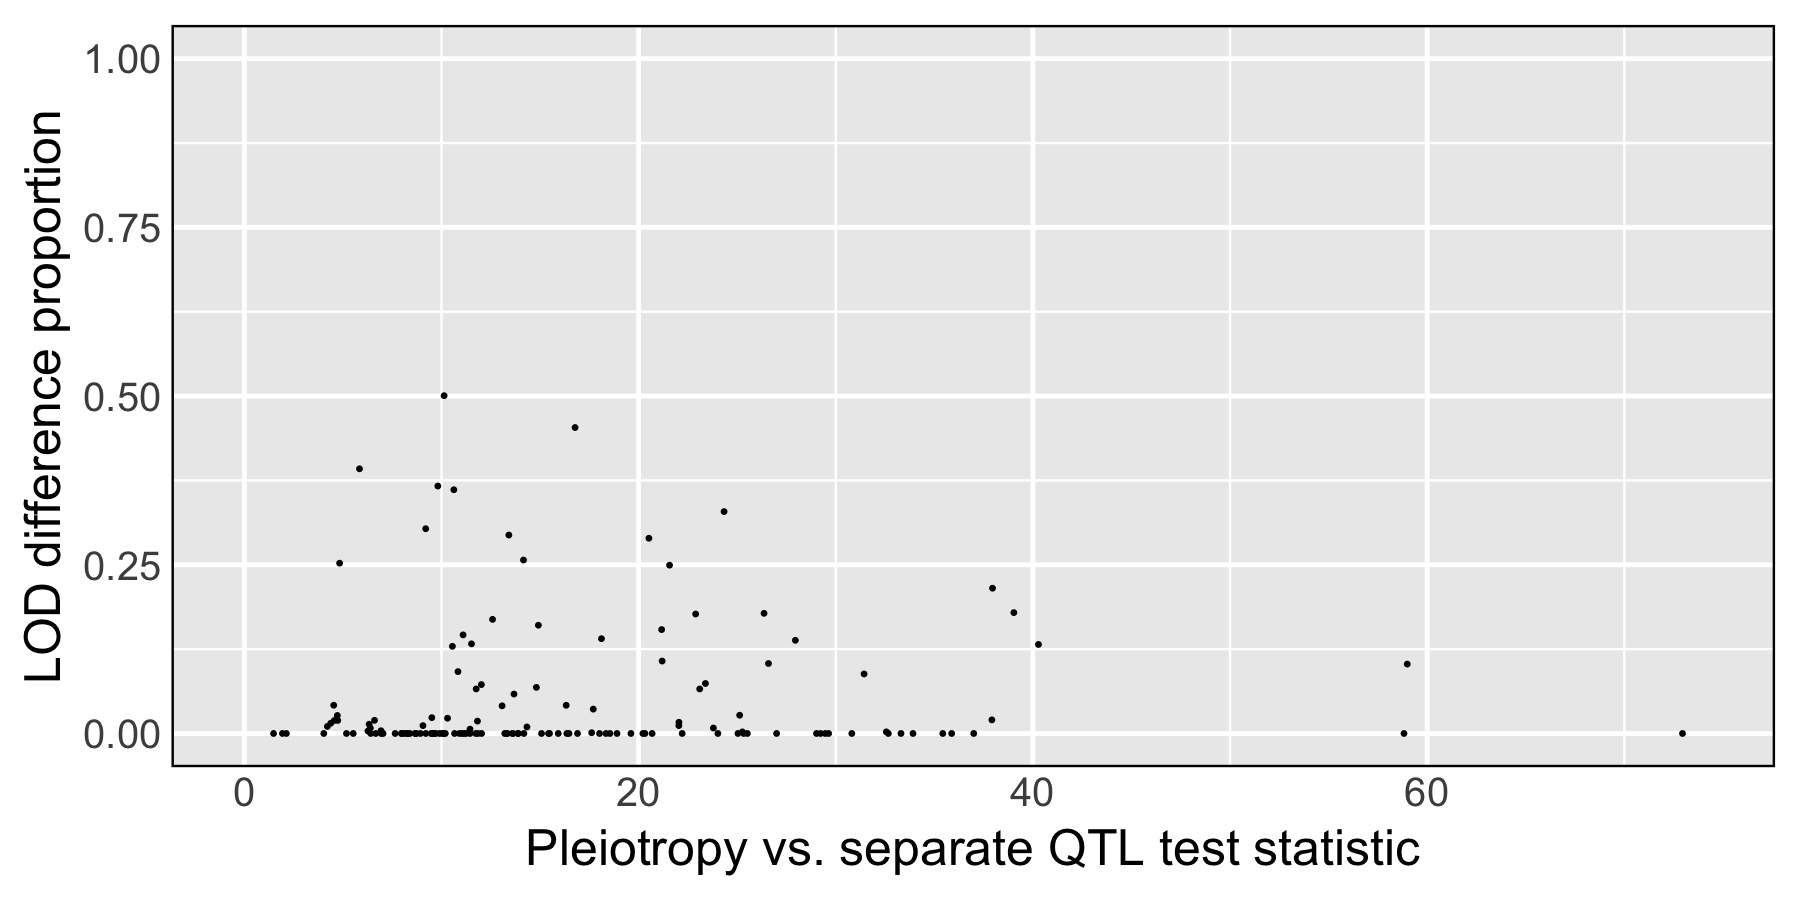
\includegraphics[width=\linewidth]{bar_12.jpg}
\caption{}\label{fig:fig_l}
\end{subfigure}

\end{figure}

\newpage
% latex table generated in R 3.5.1 by xtable 1.8-3 package
% Tue Dec 18 18:18:00 2018
\begin{longtable}{lrr}
  \caption{LOD peak positions and peak heights for 147 expression traits that map to the Chromosome 2 expression trait hotspot.}
  \label{tab:hot-annot}
\hline \\

Gene symbol & Peak position & LOD \\ 
  \hline
Mtfp1 & 163.52 & 17.79 \\ 
  Slc12a7 & 163.58 & 8.30 \\ 
  Gpa33 & 163.58 & 26.38 \\ 
  Tmem25 & 163.58 & 11.26 \\ 
  Klhl29 & 163.58 & 11.03 \\ 
  Slc9a3r1 & 163.58 & 8.40 \\ 
  Kif1c & 163.58 & 11.12 \\ 
  Gata4 & 163.58 & 8.72 \\ 
  Ppp2r5b & 163.58 & 7.80 \\ 
  Vil1 & 163.58 & 26.48 \\ 
  Aldh4a1 & 163.58 & 9.38 \\ 
  Cotl1 & 163.58 & 16.25 \\ 
  Tmprss4 & 163.58 & 18.30 \\ 
  Fhod3 & 163.58 & 17.62 \\ 
  Zfp750 & 163.58 & 7.83 \\ 
  Svop & 163.58 & 10.12 \\ 
  Abcb4 & 163.58 & 16.59 \\ 
  Ccnjl & 163.58 & 6.70 \\ 
  Sephs2 & 163.58 & 27.21 \\ 
  Pcdh1 & 163.58 & 12.48 \\ 
  Fat1 & 163.58 & 7.49 \\ 
  Sox4 & 163.58 & 14.71 \\ 
  Gm8206 & 163.58 & 11.33 \\ 
  Gm8492 & 163.58 & 10.47 \\ 
  Clcn5 & 164.02 & 10.49 \\ 
  Slc6a8 & 164.02 & 8.35 \\ 
  Bcmo1 & 164.02 & 47.31 \\ 
  Arrdc4 & 164.02 & 8.75 \\ 
  Cacnb3 & 164.02 & 47.06 \\ 
  Sec14l2 & 164.02 & 12.00 \\ 
  Pgrmc1 & 164.02 & 15.88 \\ 
  Baiap2l2 & 164.02 & 20.33 \\ 
  Recql5 & 164.02 & 33.97 \\ 
  Cpd & 164.02 & 13.70 \\ 
  Degs2 & 164.02 & 15.20 \\ 
  Muc13 & 164.02 & 18.91 \\ 
  Clic5 & 164.02 & 10.39 \\ 
  Tff3 & 164.02 & 16.38 \\ 
  Myo7b & 164.02 & 13.70 \\ 
  Afg3l2 & 164.02 & 19.12 \\ 
  Sema4g & 164.02 & 23.39 \\ 
  Agap2 & 164.02 & 33.99 \\ 
  Plxna2 & 164.02 & 8.61 \\ 
  Aldob & 164.02 & 20.99 \\ 
  Epb4.1l4b & 164.02 & 9.21 \\ 
  Sel1l3 & 164.02 & 17.92 \\ 
  Sult1b1 & 164.02 & 17.63 \\ 
  Hpgds & 164.02 & 31.14 \\ 
  Ush1c & 164.02 & 21.90 \\ 
  Calml4 & 164.02 & 12.62 \\ 
  Fam83b & 164.02 & 16.12 \\ 
  Myo15b & 164.02 & 71.57 \\ 
  Inpp5j & 164.02 & 11.57 \\ 
  Ttyh2 & 164.02 & 15.20 \\ 
  Cdhr2 & 164.02 & 30.00 \\ 
  Myrf & 164.02 & 37.55 \\ 
  Sh3bp4 & 164.02 & 9.04 \\ 
  Vgf & 164.02 & 15.05 \\ 
  Grtp1 & 164.02 & 23.88 \\ 
  B4galnt3 & 164.02 & 20.43 \\ 
  Gucy2c & 164.02 & 12.02 \\ 
  Smim5 & 164.02 & 18.20 \\ 
  Nrip1 & 164.02 & 9.50 \\ 
  Clrn3 & 164.02 & 20.13 \\ 
  Acot4 & 164.02 & 12.17 \\ 
  Hunk & 164.02 & 18.50 \\ 
  Zbtb16 & 164.02 & 6.69 \\ 
  Osgin1 & 164.02 & 13.51 \\ 
  Zfp541 & 164.02 & 25.28 \\ 
  2610042L04Rik & 164.02 & 8.14 \\ 
  Gm9429 & 164.02 & 9.13 \\ 
  Agxt2 & 164.02 & 14.54 \\ 
  Gm17147 & 164.02 & 26.94 \\ 
  Gm8281 & 164.02 & 8.40 \\ 
  Ddx23 & 164.03 & 9.29 \\ 
  Map2k6 & 164.03 & 18.54 \\ 
  Npr1 & 164.03 & 9.68 \\ 
  Hdac6 & 164.03 & 11.28 \\ 
  Vav3 & 164.03 & 13.51 \\ 
  Atp11b & 164.03 & 11.77 \\ 
  Aadat & 164.03 & 8.08 \\ 
  Tmem19 & 164.03 & 20.60 \\ 
  Gbp4 & 164.03 & 7.14 \\ 
  Papola & 164.03 & 12.14 \\ 
  Als2 & 164.03 & 18.35 \\ 
  Sult1d1 & 164.03 & 11.23 \\ 
  Myo6 & 164.03 & 10.27 \\ 
  Dnajc22 & 164.03 & 13.72 \\ 
  Unc5d & 164.03 & 6.96 \\ 
  Gm3095 & 164.03 & 10.90 \\ 
  Gm26886 & 164.03 & 8.76 \\ 
  Eps8 & 164.06 & 12.49 \\ 
  Ddc & 164.06 & 13.61 \\ 
  Fras1 & 164.06 & 10.06 \\ 
  Card11 & 164.06 & 7.20 \\ 
  Glyat & 164.06 & 10.79 \\ 
  Pipox & 164.08 & 15.90 \\ 
  Iyd & 164.08 & 23.23 \\ 
  Man1a & 164.26 & 8.77 \\ 
  Cdc42ep4 & 164.26 & 8.11 \\ 
  Ppara & 164.26 & 8.84 \\ 
  Galr1 & 164.26 & 10.10 \\ 
  Ctdsp1 & 164.26 & 7.13 \\ 
  Eif2ak3 & 164.26 & 8.93 \\ 
  Misp & 164.26 & 9.24 \\ 
  Sun1 & 164.26 & 7.35 \\ 
  Kctd8 & 164.26 & 9.76 \\ 
  Dcaf12l1 & 164.26 & 8.95 \\ 
  4930539E08Rik & 164.26 & 8.25 \\ 
  Slc29a4 & 164.26 & 7.94 \\ 
  Gm3239 & 164.26 & 9.21 \\ 
  Gm3629 & 164.26 & 9.77 \\ 
  Gm3252 & 164.26 & 9.87 \\ 
  Gm3002 & 164.26 & 7.62 \\ 
  Ctsh & 164.29 & 9.76 \\ 
  Dao & 164.29 & 7.06 \\ 
  Ak7 & 164.31 & 10.07 \\ 
  Pcp4l1 & 164.35 & 9.11 \\ 
  Gm12929 & 164.62 & 37.80 \\ 
  Mgat1 & 164.63 & 10.10 \\ 
  Atg7 & 164.76 & 7.82 \\ 
  Gm11549 & 165.05 & 10.23 \\ 
  Ccdc111 & 165.12 & 7.77 \\ 
  Fam20a & 165.15 & 7.59 \\ 
  Oscp1 & 165.16 & 7.99 \\ 
  Dsc2 & 165.28 & 8.06 \\ 
  Adam10 & 165.28 & 9.73 \\ 
  Plb1 & 165.28 & 8.85 \\ 
  Ccdc89 & 165.28 & 7.84 \\ 
  9930013L23Rik & 165.28 & 7.93 \\ 
  Gm13648 & 165.28 & 7.08 \\ 
  Igfbp4 & 165.45 & 8.68 \\ 
  Ldlrap1 & 165.45 & 7.18 \\ 
  Cdh18 & 165.45 & 7.96 \\ 
  Arhgef10l & 165.46 & 7.57 \\ 
  Cib3 & 165.48 & 8.70 \\ 
  Macf1 & 165.57 & 9.10 \\ 
  Fam63b & 165.58 & 8.33 \\ 
  1190002N15Rik & 165.63 & 9.02 \\ 
  Bcl2l14 & 165.71 & 7.54 \\ 
  Hist2h2be & 165.88 & 8.96 \\ 
  Gm6428 & 165.89 & 7.32 \\ 
  Dennd5b & 166.18 & 9.42 \\ 
  Gm12168 & 166.18 & 7.77 \\ 
  Gm12230 & 166.42 & 7.46 \\ 
  Acat3 & 166.61 & 7.17 \\ 
  Gpr20 & 166.84 & 8.41 \\ 
   \hline
\end{longtable}

\end{document}
